\section{Screenshots des AppHost}
\label{sec:apphost_screenshots}

Zur Veranschaulichung der in Abschnitt~\ref{sec:apps} aufgeführten Applikationen zeigt dieser Anhang eine Auswahl an Bildschirmaufnahmen des laufenden Systems. Sie dokumentieren exemplarisch den Zustand einzelner Dienste sowie deren Monitoring zum Zeitpunkt der Erstellung.

\begin{figure}[htbp]
    \centering
    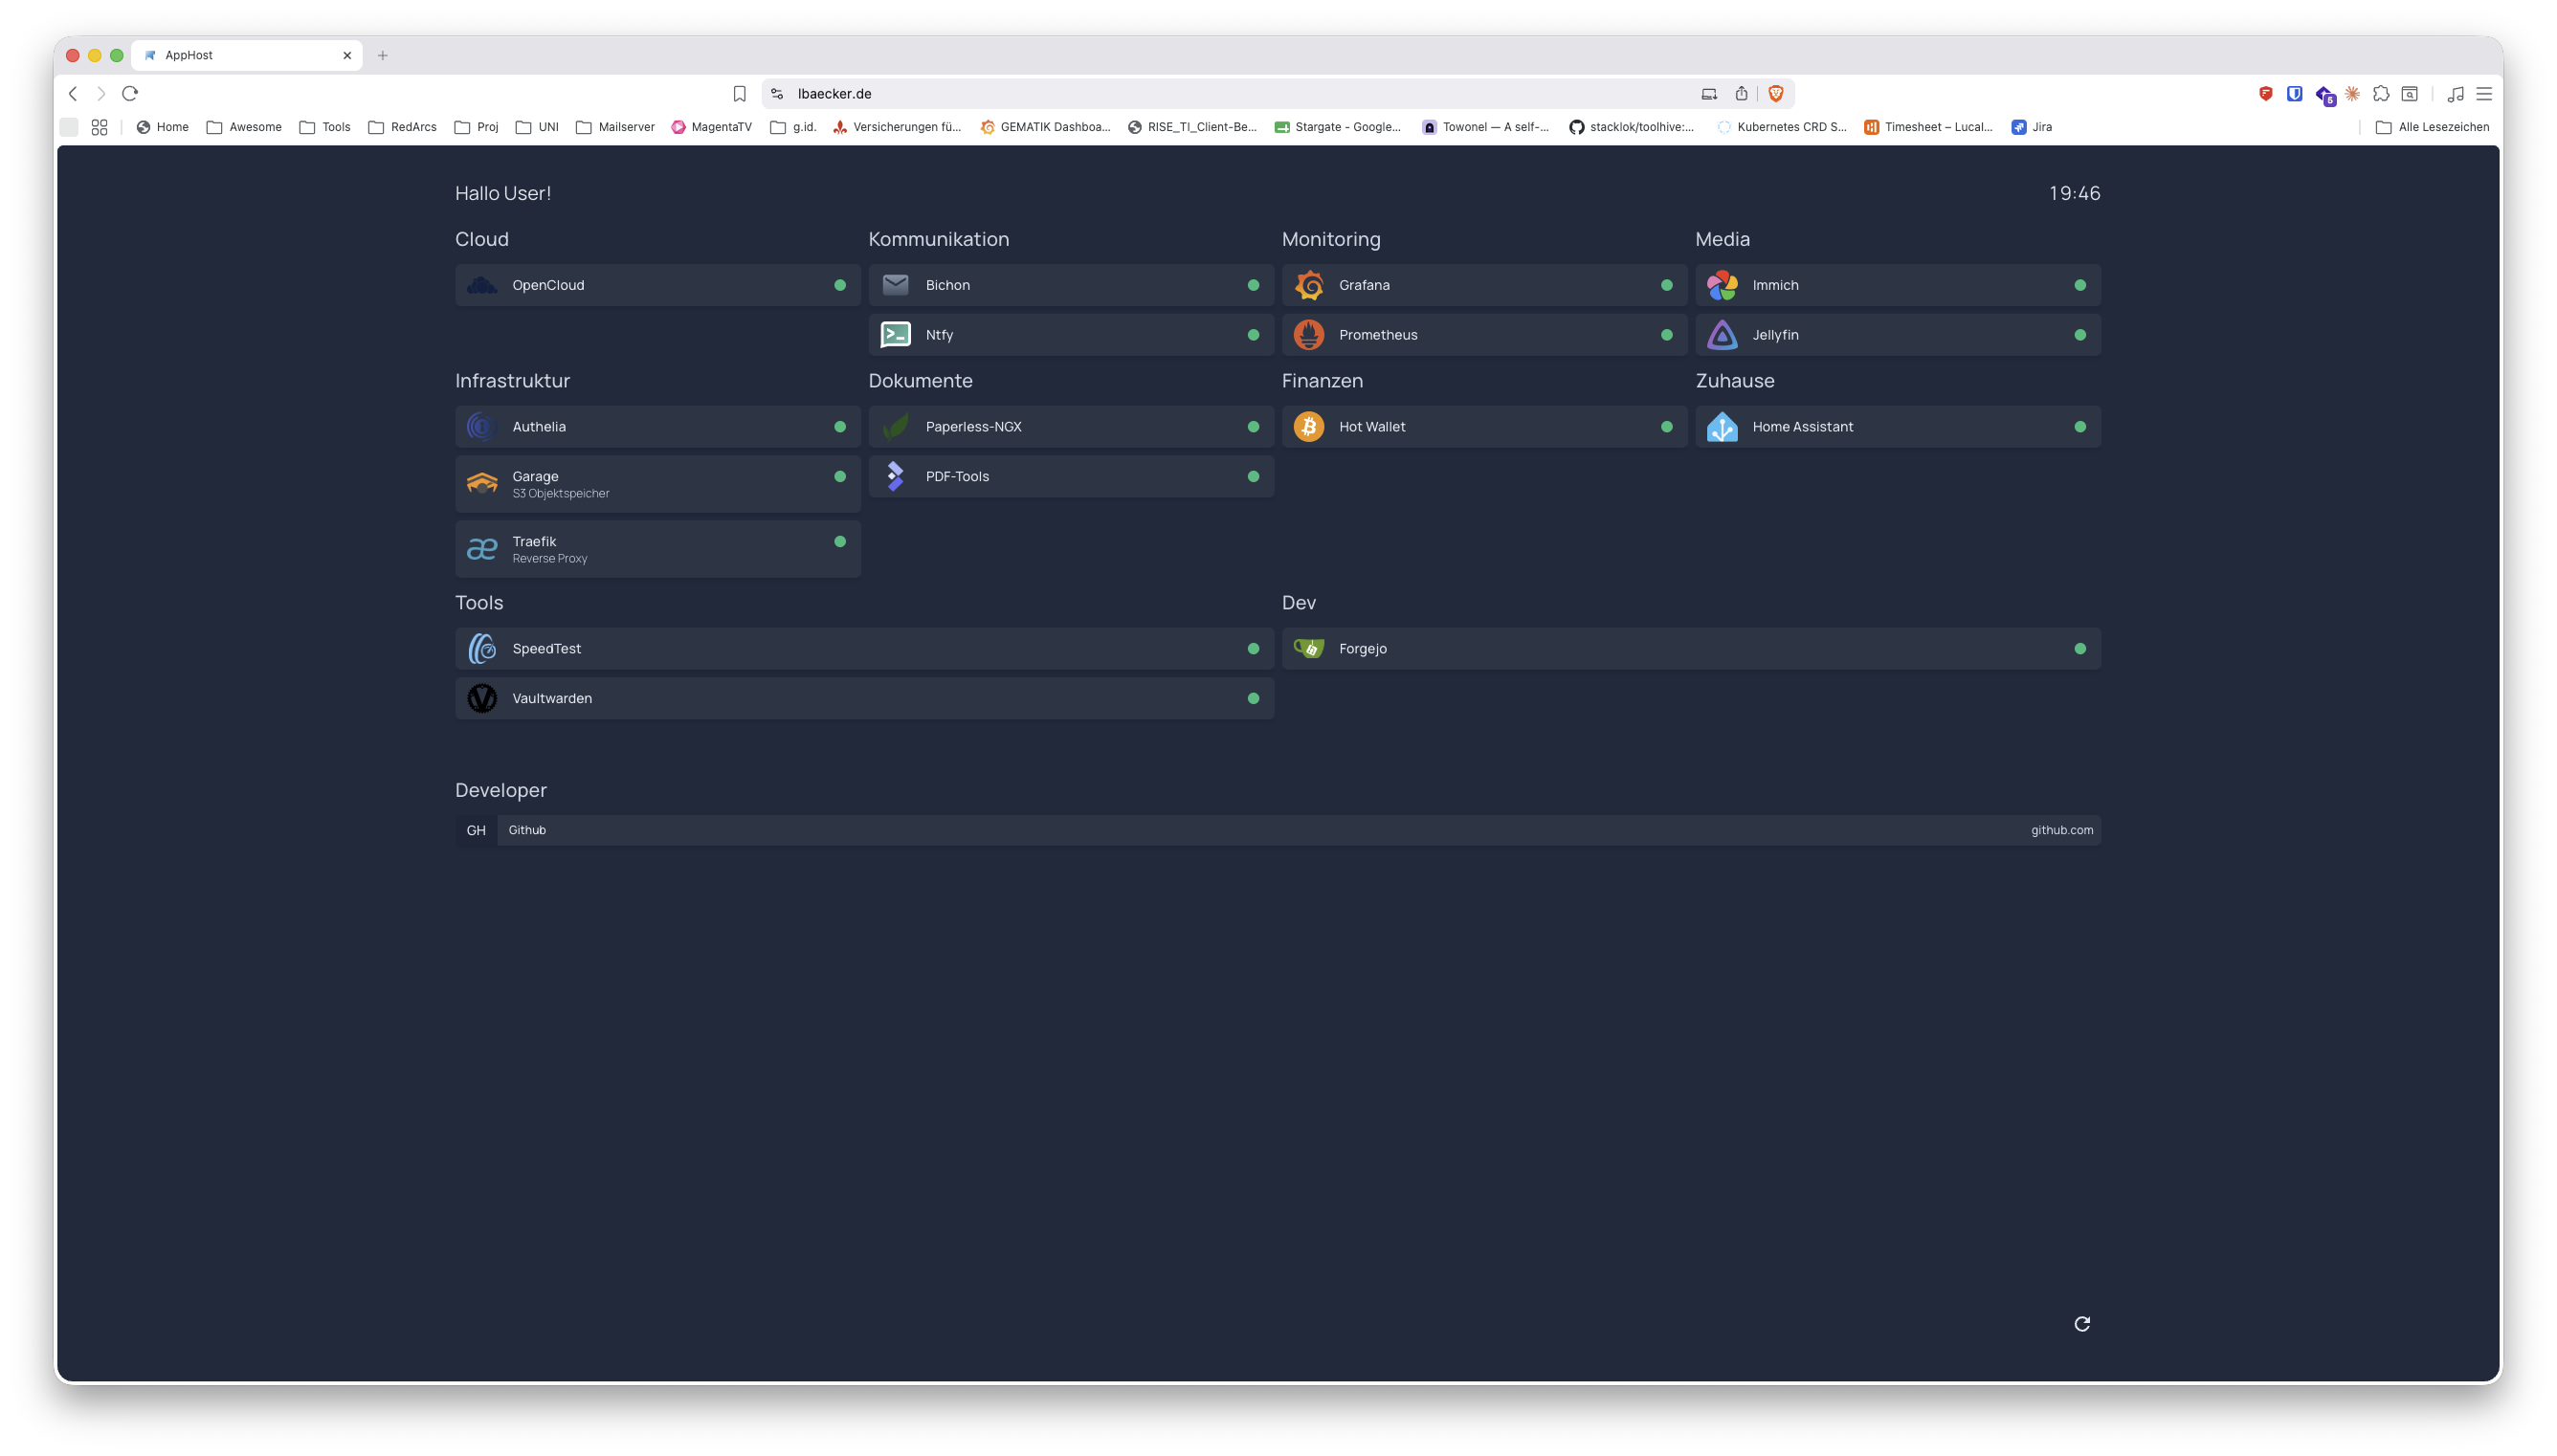
\includegraphics[width=0.9\textwidth]{Doku/Apphost/bilder/homepage_dashboard.png}
    \caption{Homepage-Dashboard mit Übersicht aller Dienste, gruppiert nach Kategorie. Der grüne Punkt neben jedem Eintrag zeigt den erreichten Online-Status an. Quelle: Eigene Bildschirmaufnahme.}
    \label{fig:apphost_homepage}
\end{figure}

\begin{figure}[htbp]
    \centering
    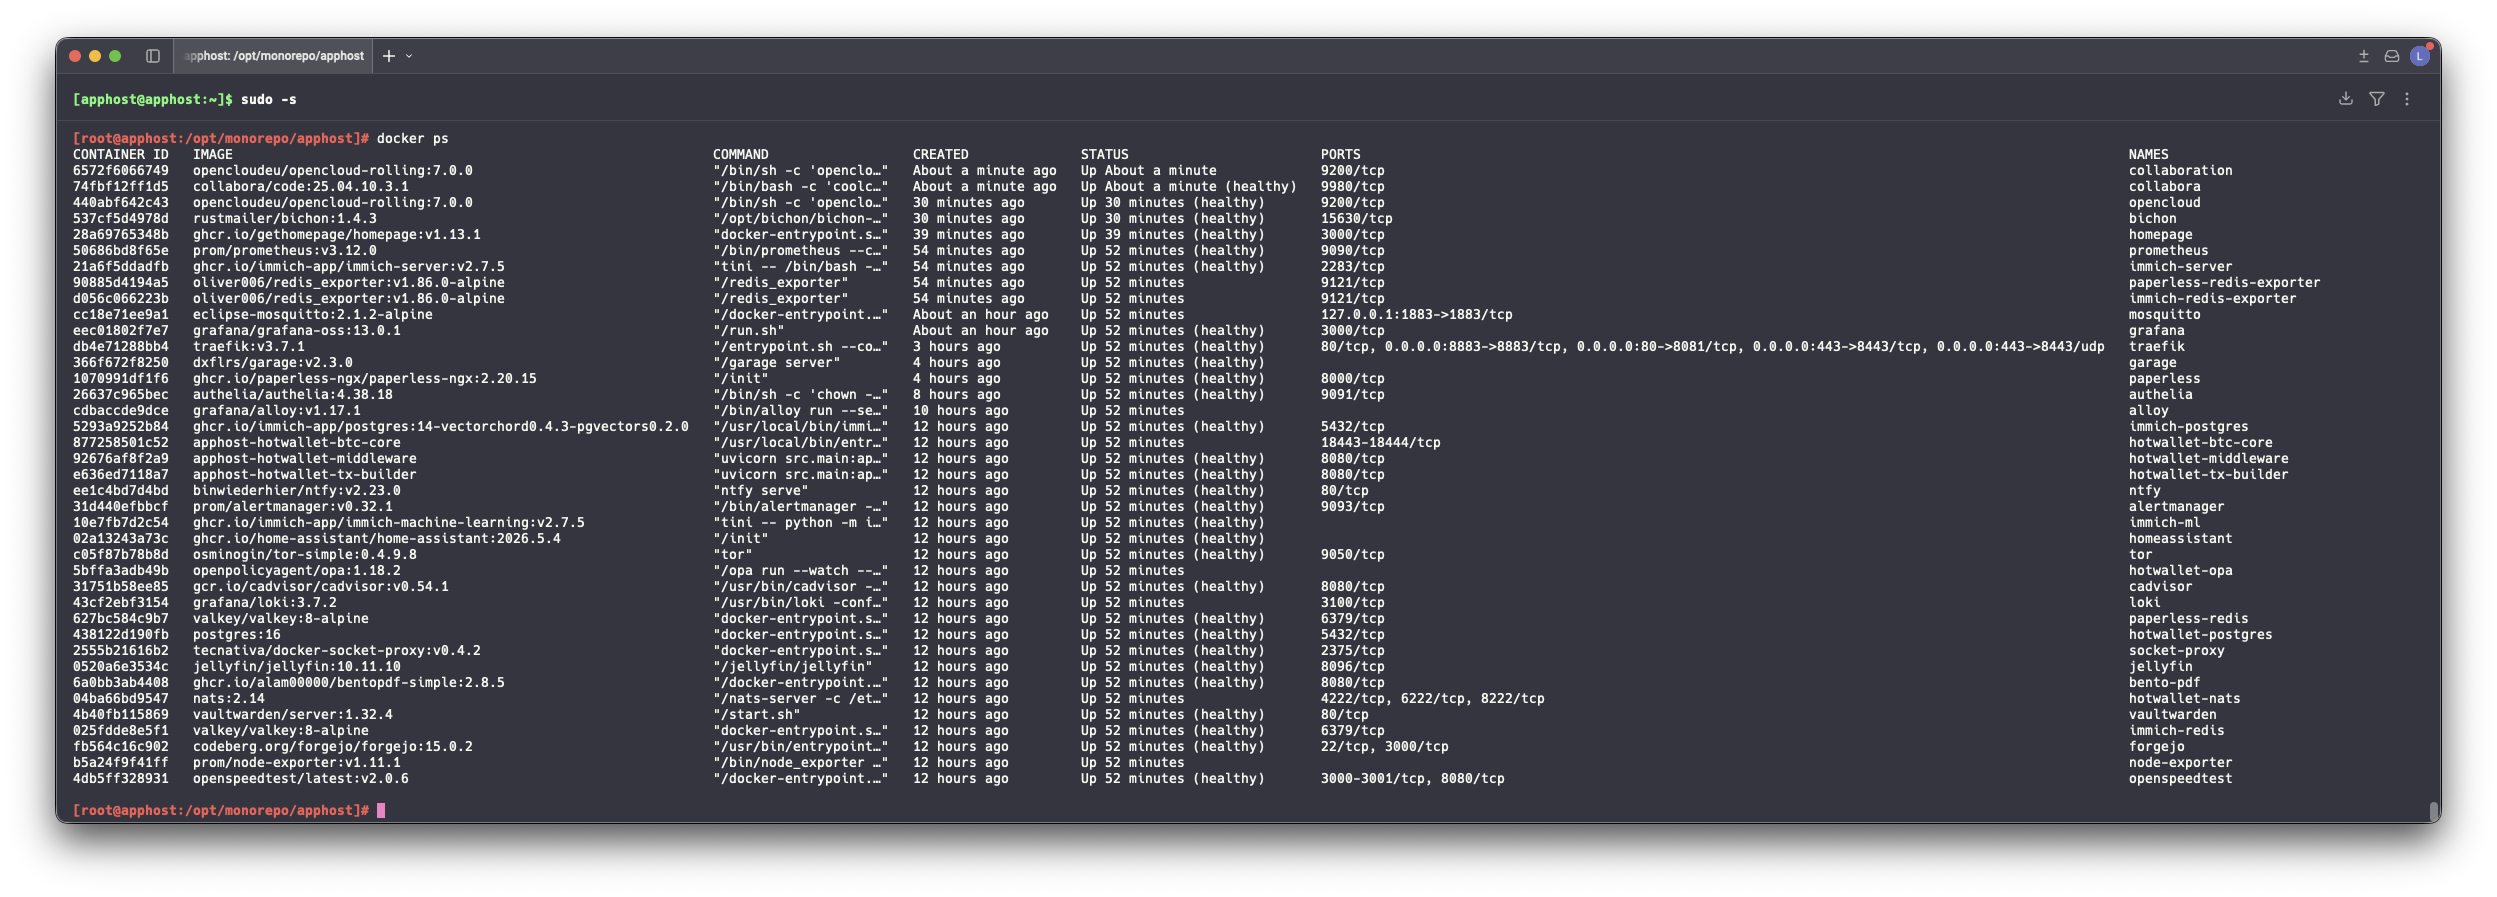
\includegraphics[width=0.9\textwidth]{Doku/Apphost/bilder/docker_ps_overview.png}
    \caption{Ausgabe von \texttt{docker ps} auf dem AppHost. Alle Container laufen im gemeinsamen Monorepo-Deployment unter \texttt{/opt/monorepo/apphost} und melden überwiegend den Status \texttt{healthy}. Quelle: Eigene Bildschirmaufnahme.}
    \label{fig:apphost_docker_ps}
\end{figure}

\begin{figure}[htbp]
    \centering
    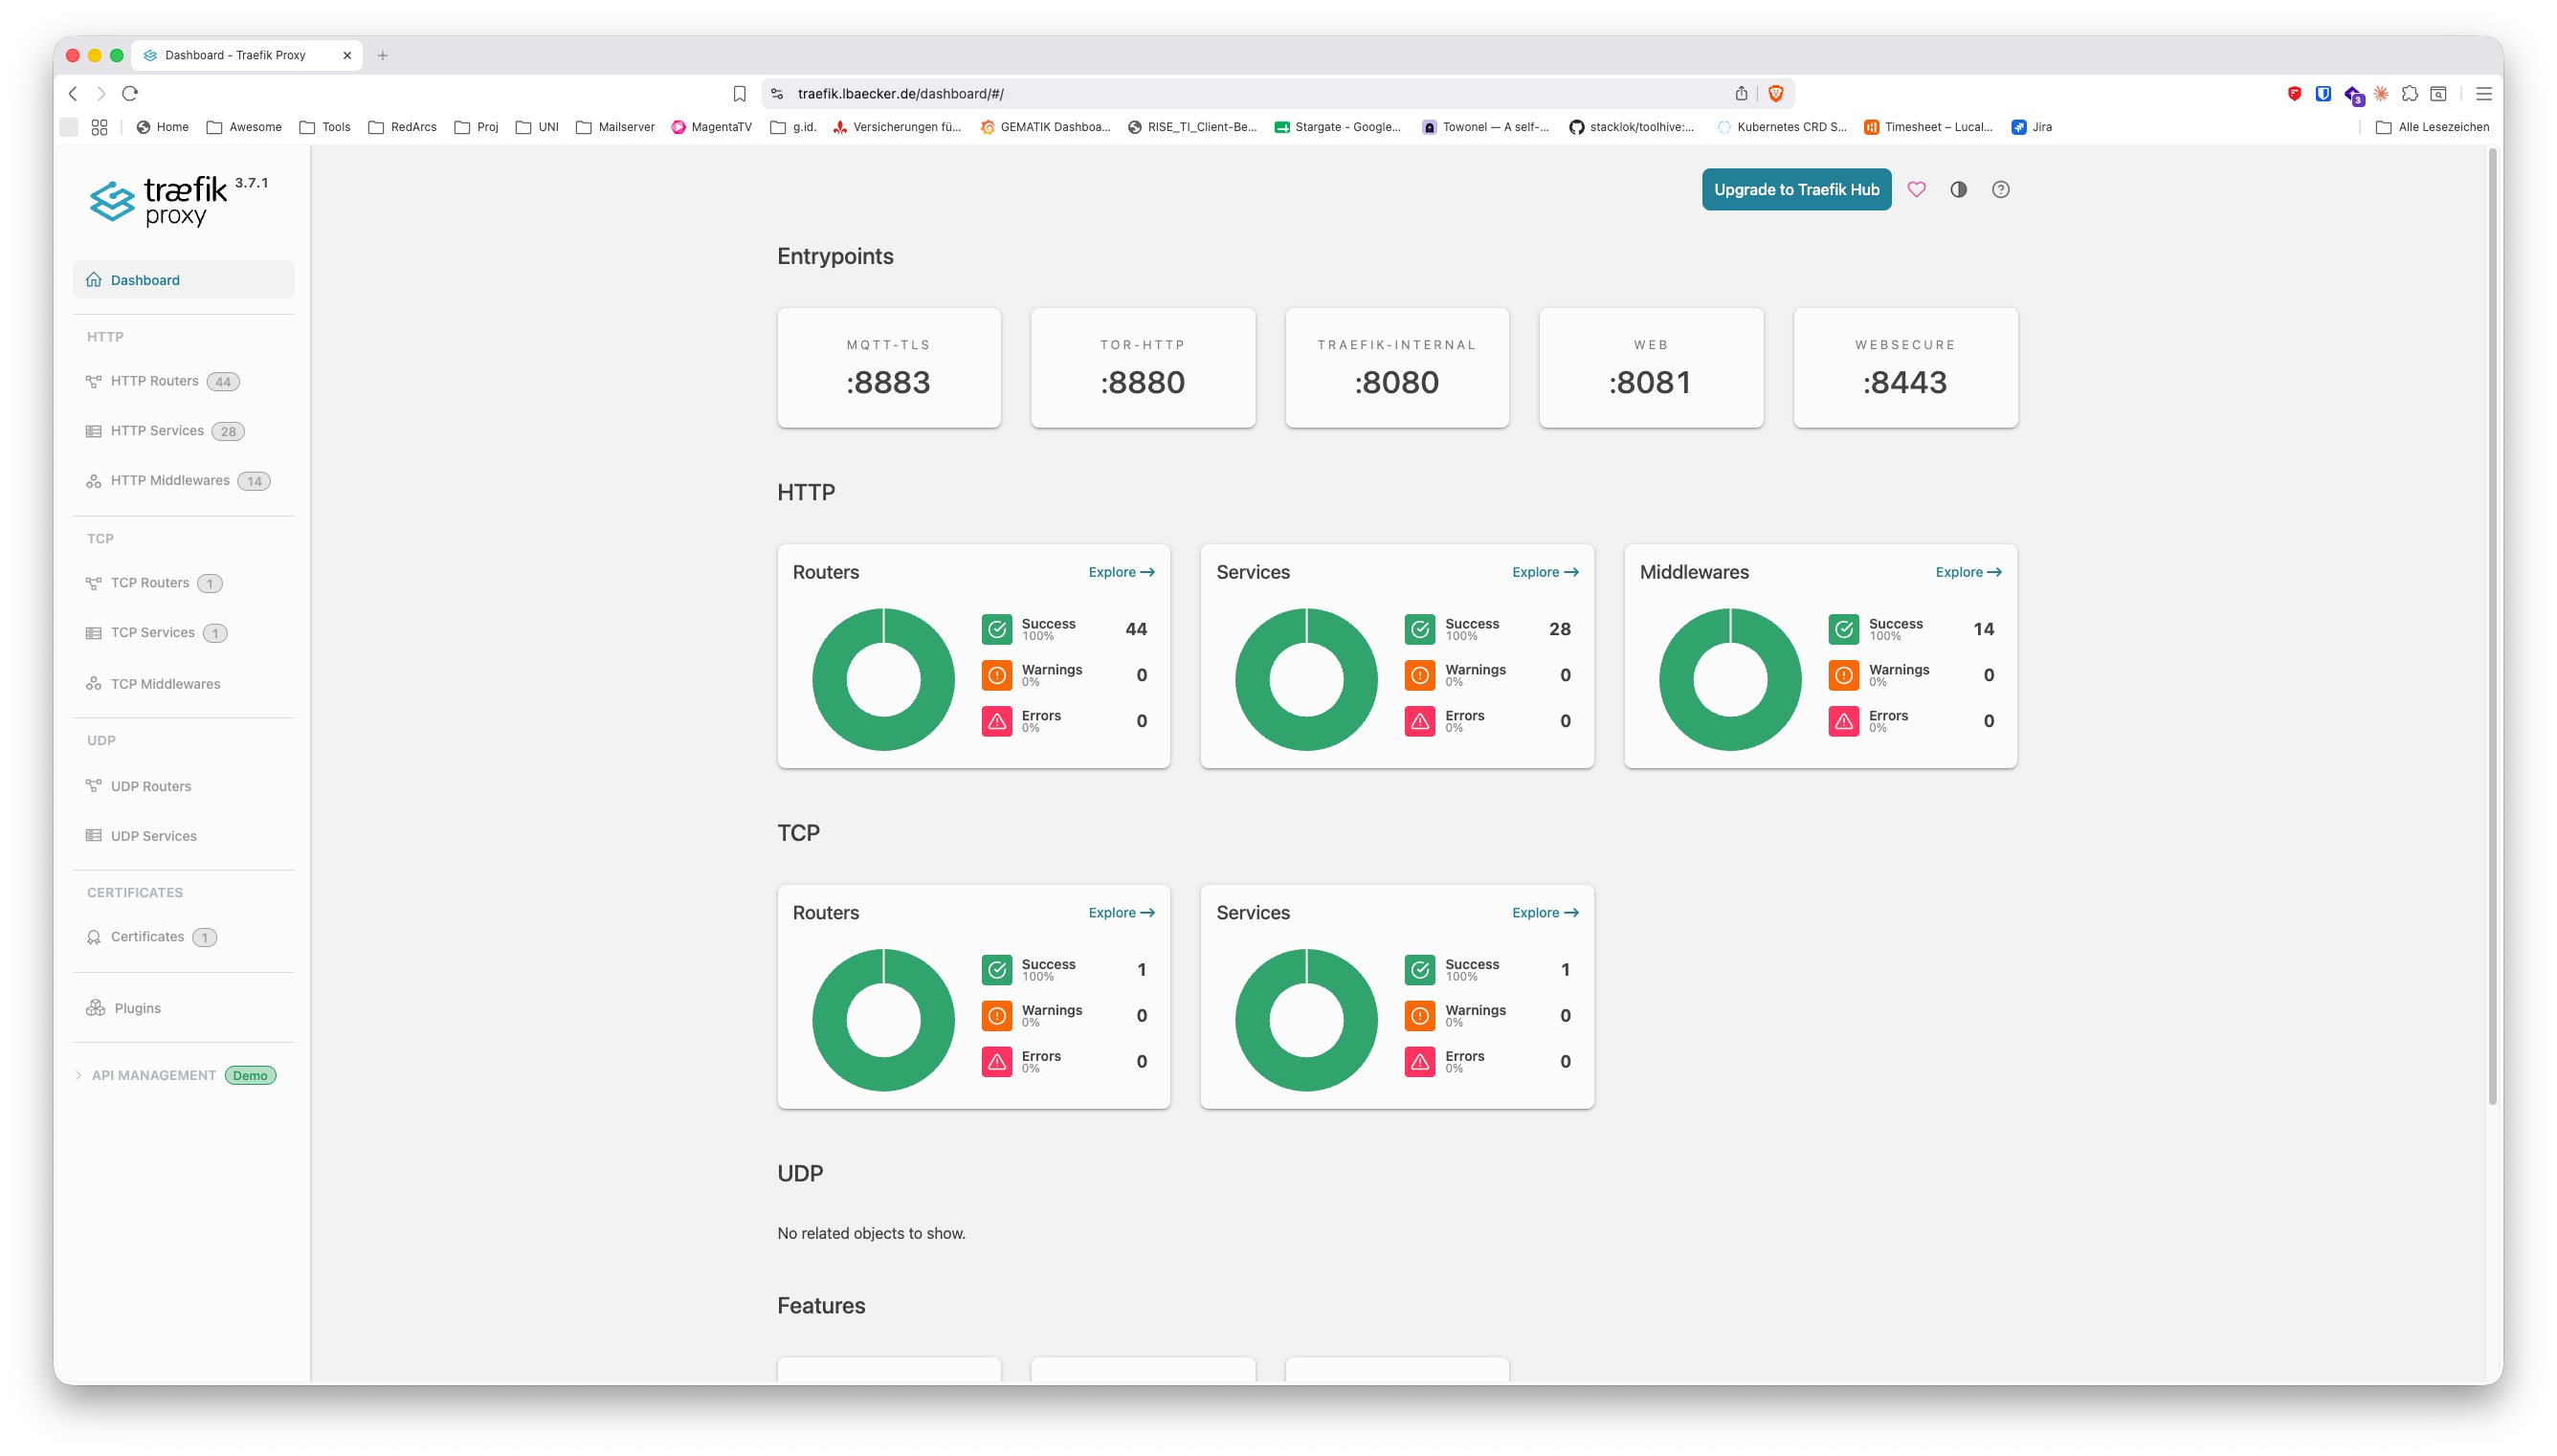
\includegraphics[width=0.9\textwidth]{Doku/Apphost/bilder/traefik_dashboard.png}
    \caption{Dashboard des Traefik-Reverse-Proxys mit den konfigurierten Entrypoints (u.\,a. \texttt{web}, \texttt{websecure}, \texttt{tor-http}) sowie einer Erfolgsübersicht der \acs{HTTP}- und \acs{TCP}-Router, -Services und -Middlewares. Quelle: Eigene Bildschirmaufnahme.}
    \label{fig:apphost_traefik}
\end{figure}

\begin{figure}[htbp]
    \centering
    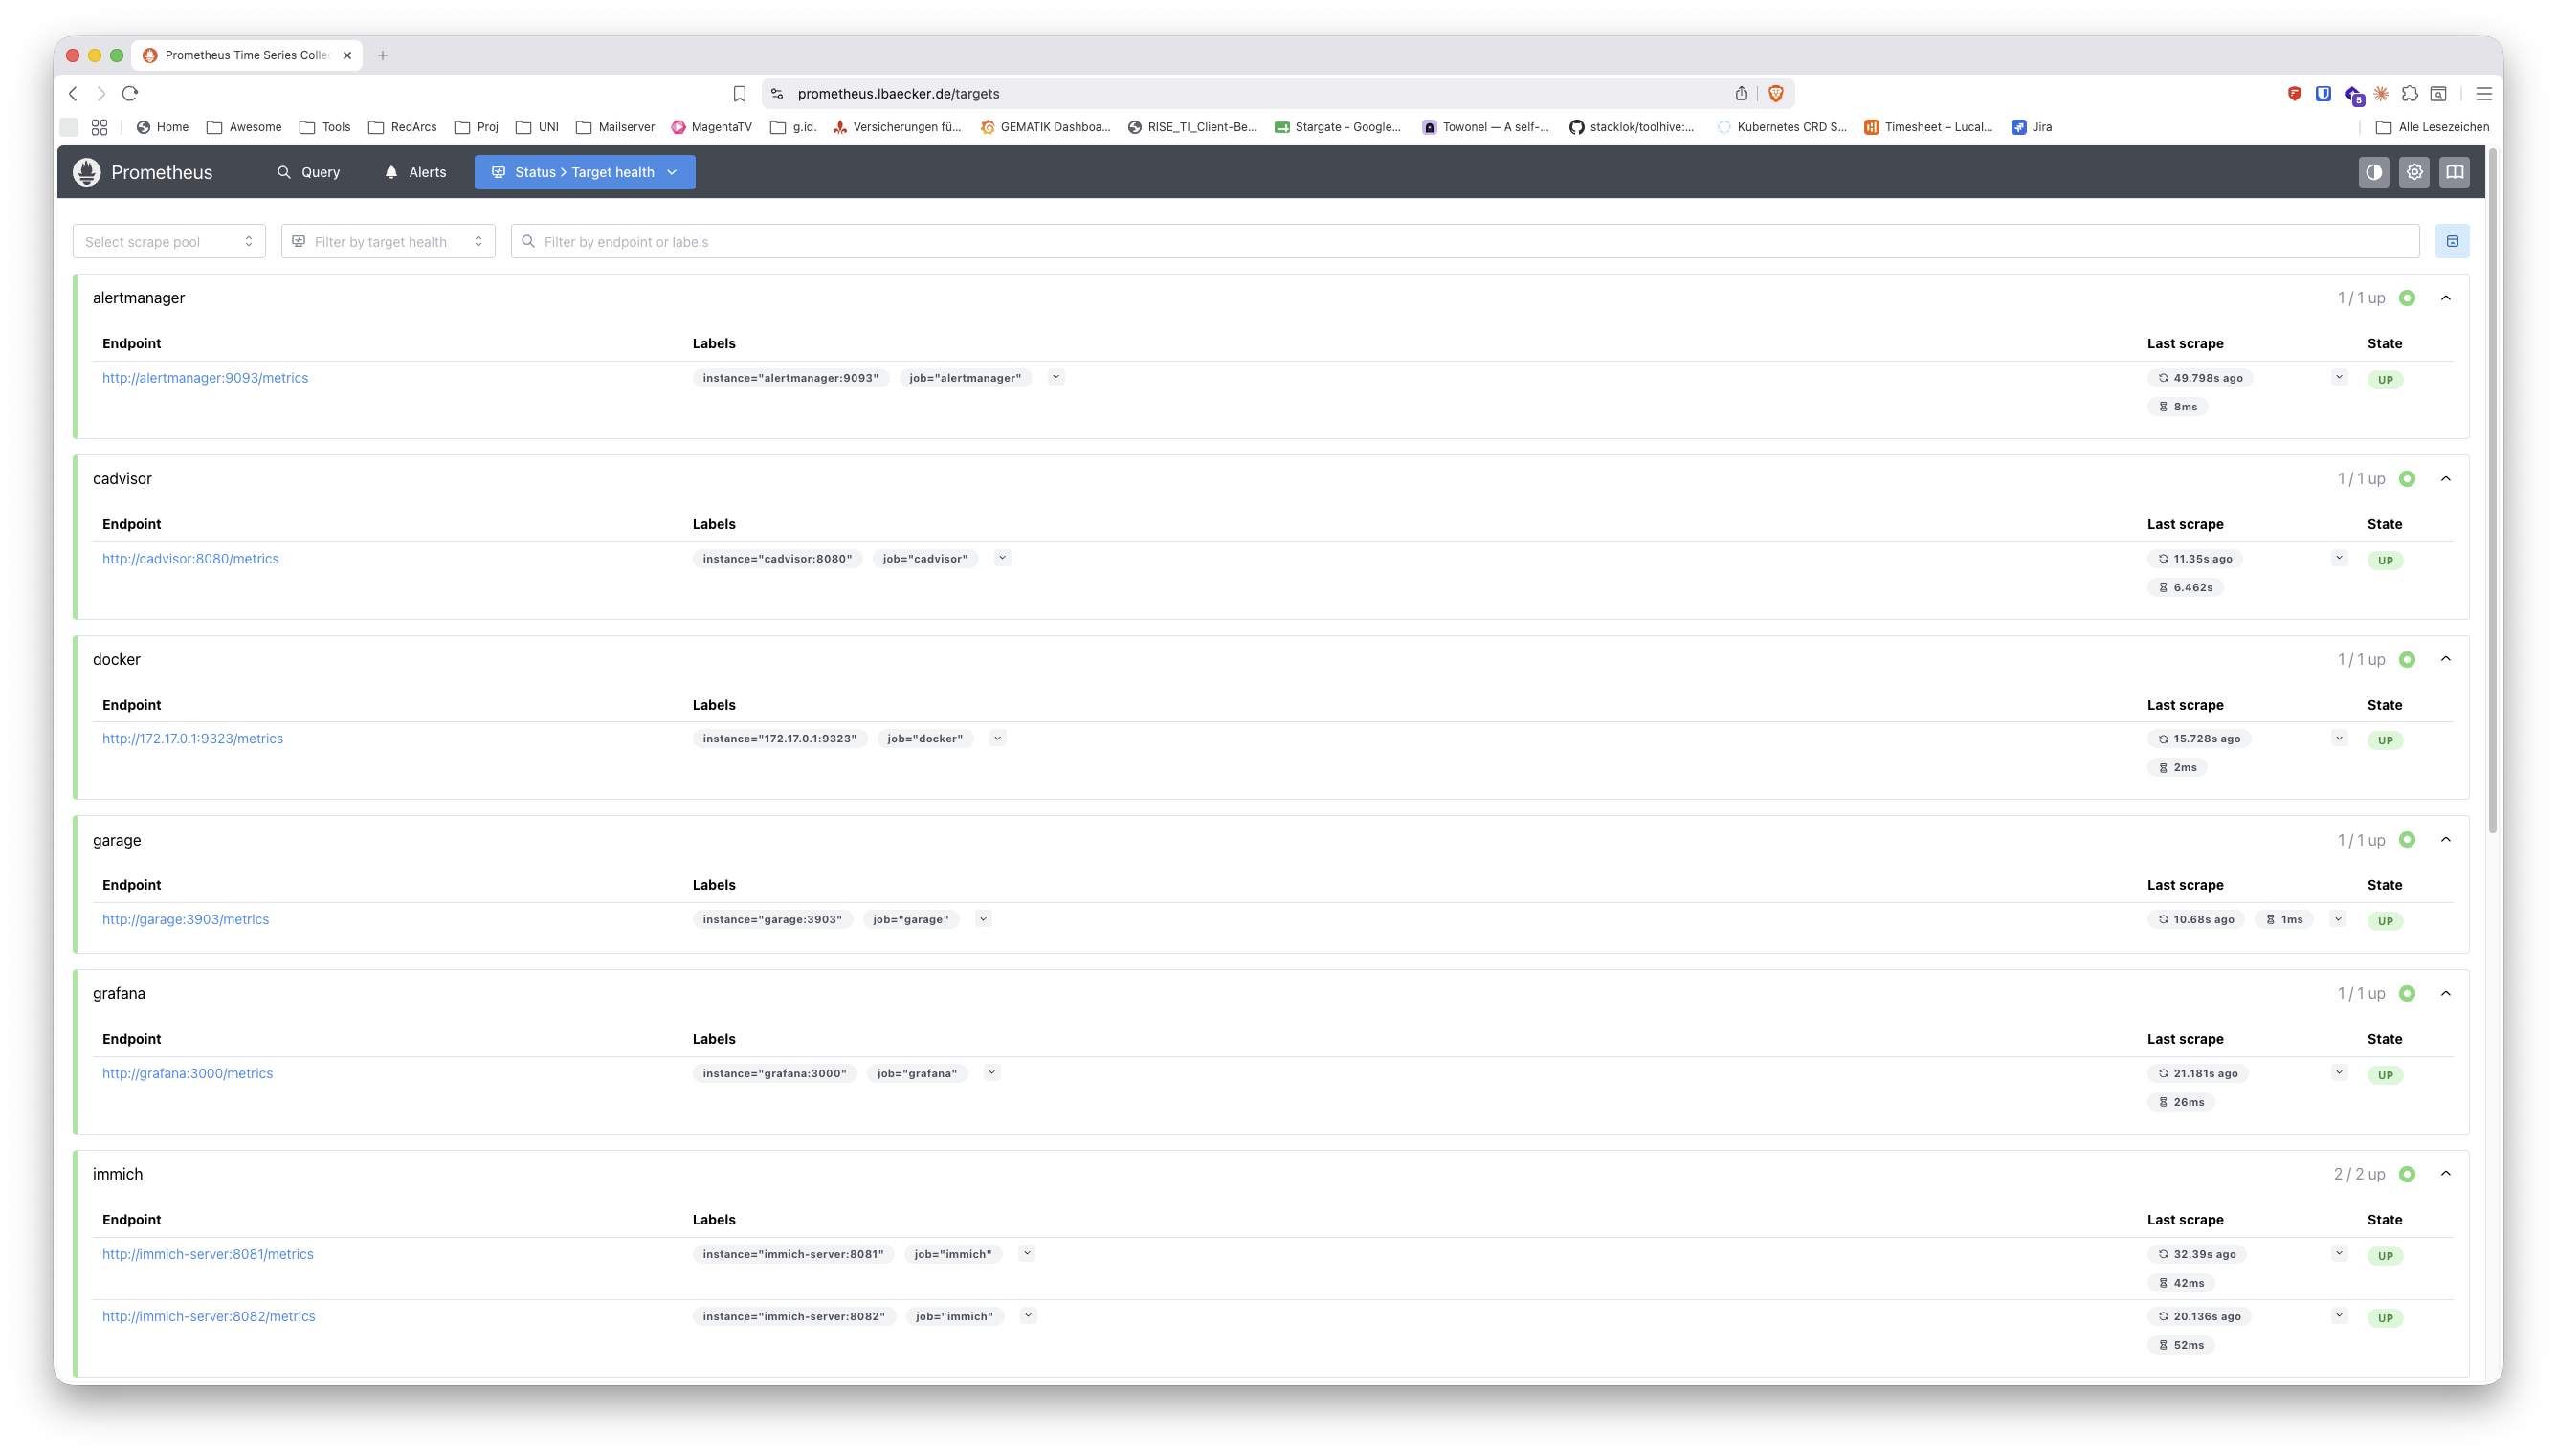
\includegraphics[width=0.9\textwidth]{Doku/Apphost/bilder/prometheus_targets.png}
    \caption{Prometheus-Statusseite \enquote{Target health}, welche die Erreichbarkeit der gescrapten Exporter (u.\,a. Alertmanager, cAdvisor, Garage, Grafana, Immich) mit Zeitstempel des letzten Scrapes anzeigt. Quelle: Eigene Bildschirmaufnahme.}
    \label{fig:apphost_prometheus_targets}
\end{figure}

\begin{figure}[htbp]
    \centering
    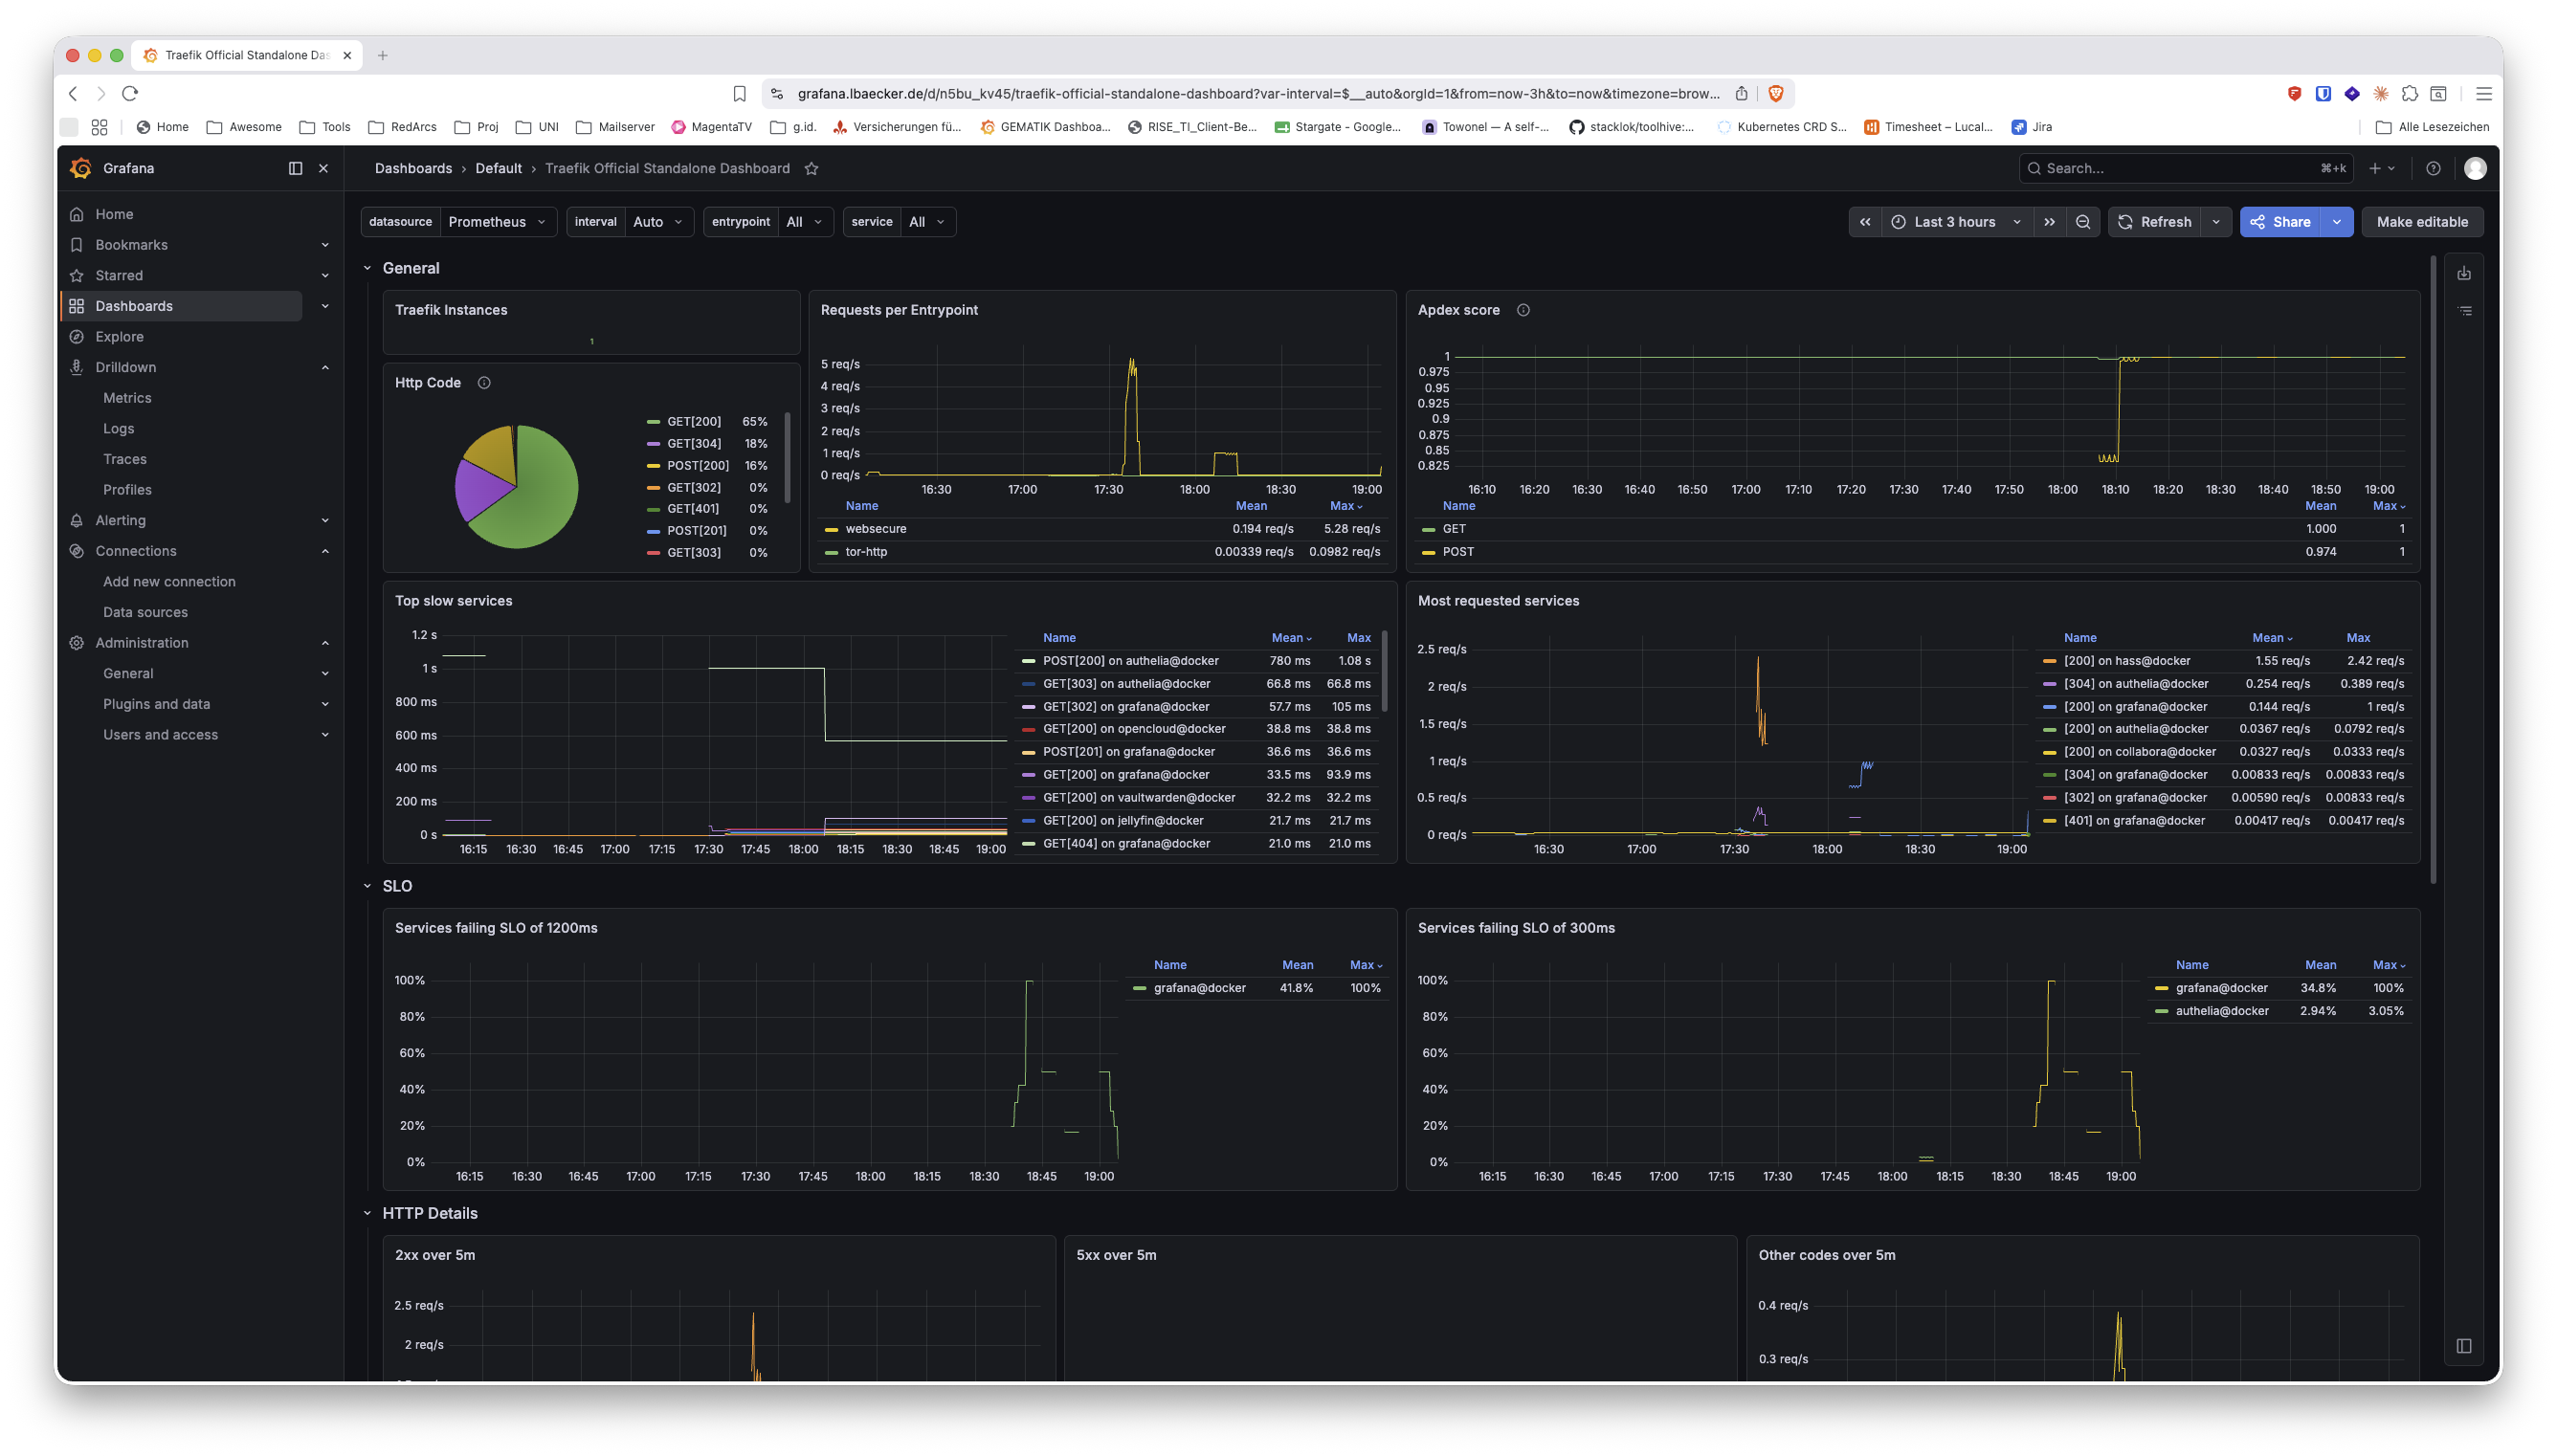
\includegraphics[width=0.9\textwidth]{Doku/Apphost/bilder/grafana_traefik_dashboard.png}
    \caption{Grafana-Dashboard \enquote{Traefik Official Standalone Dashboard} mit Request-Raten, \acs{HTTP}-Statuscodes, langsamsten Diensten sowie der Einhaltung der definierten Latenz-Schwellenwerte je Dienst. Quelle: Eigene Bildschirmaufnahme.}
    \label{fig:apphost_grafana_traefik}
\end{figure}

\begin{figure}[htbp]
    \centering
    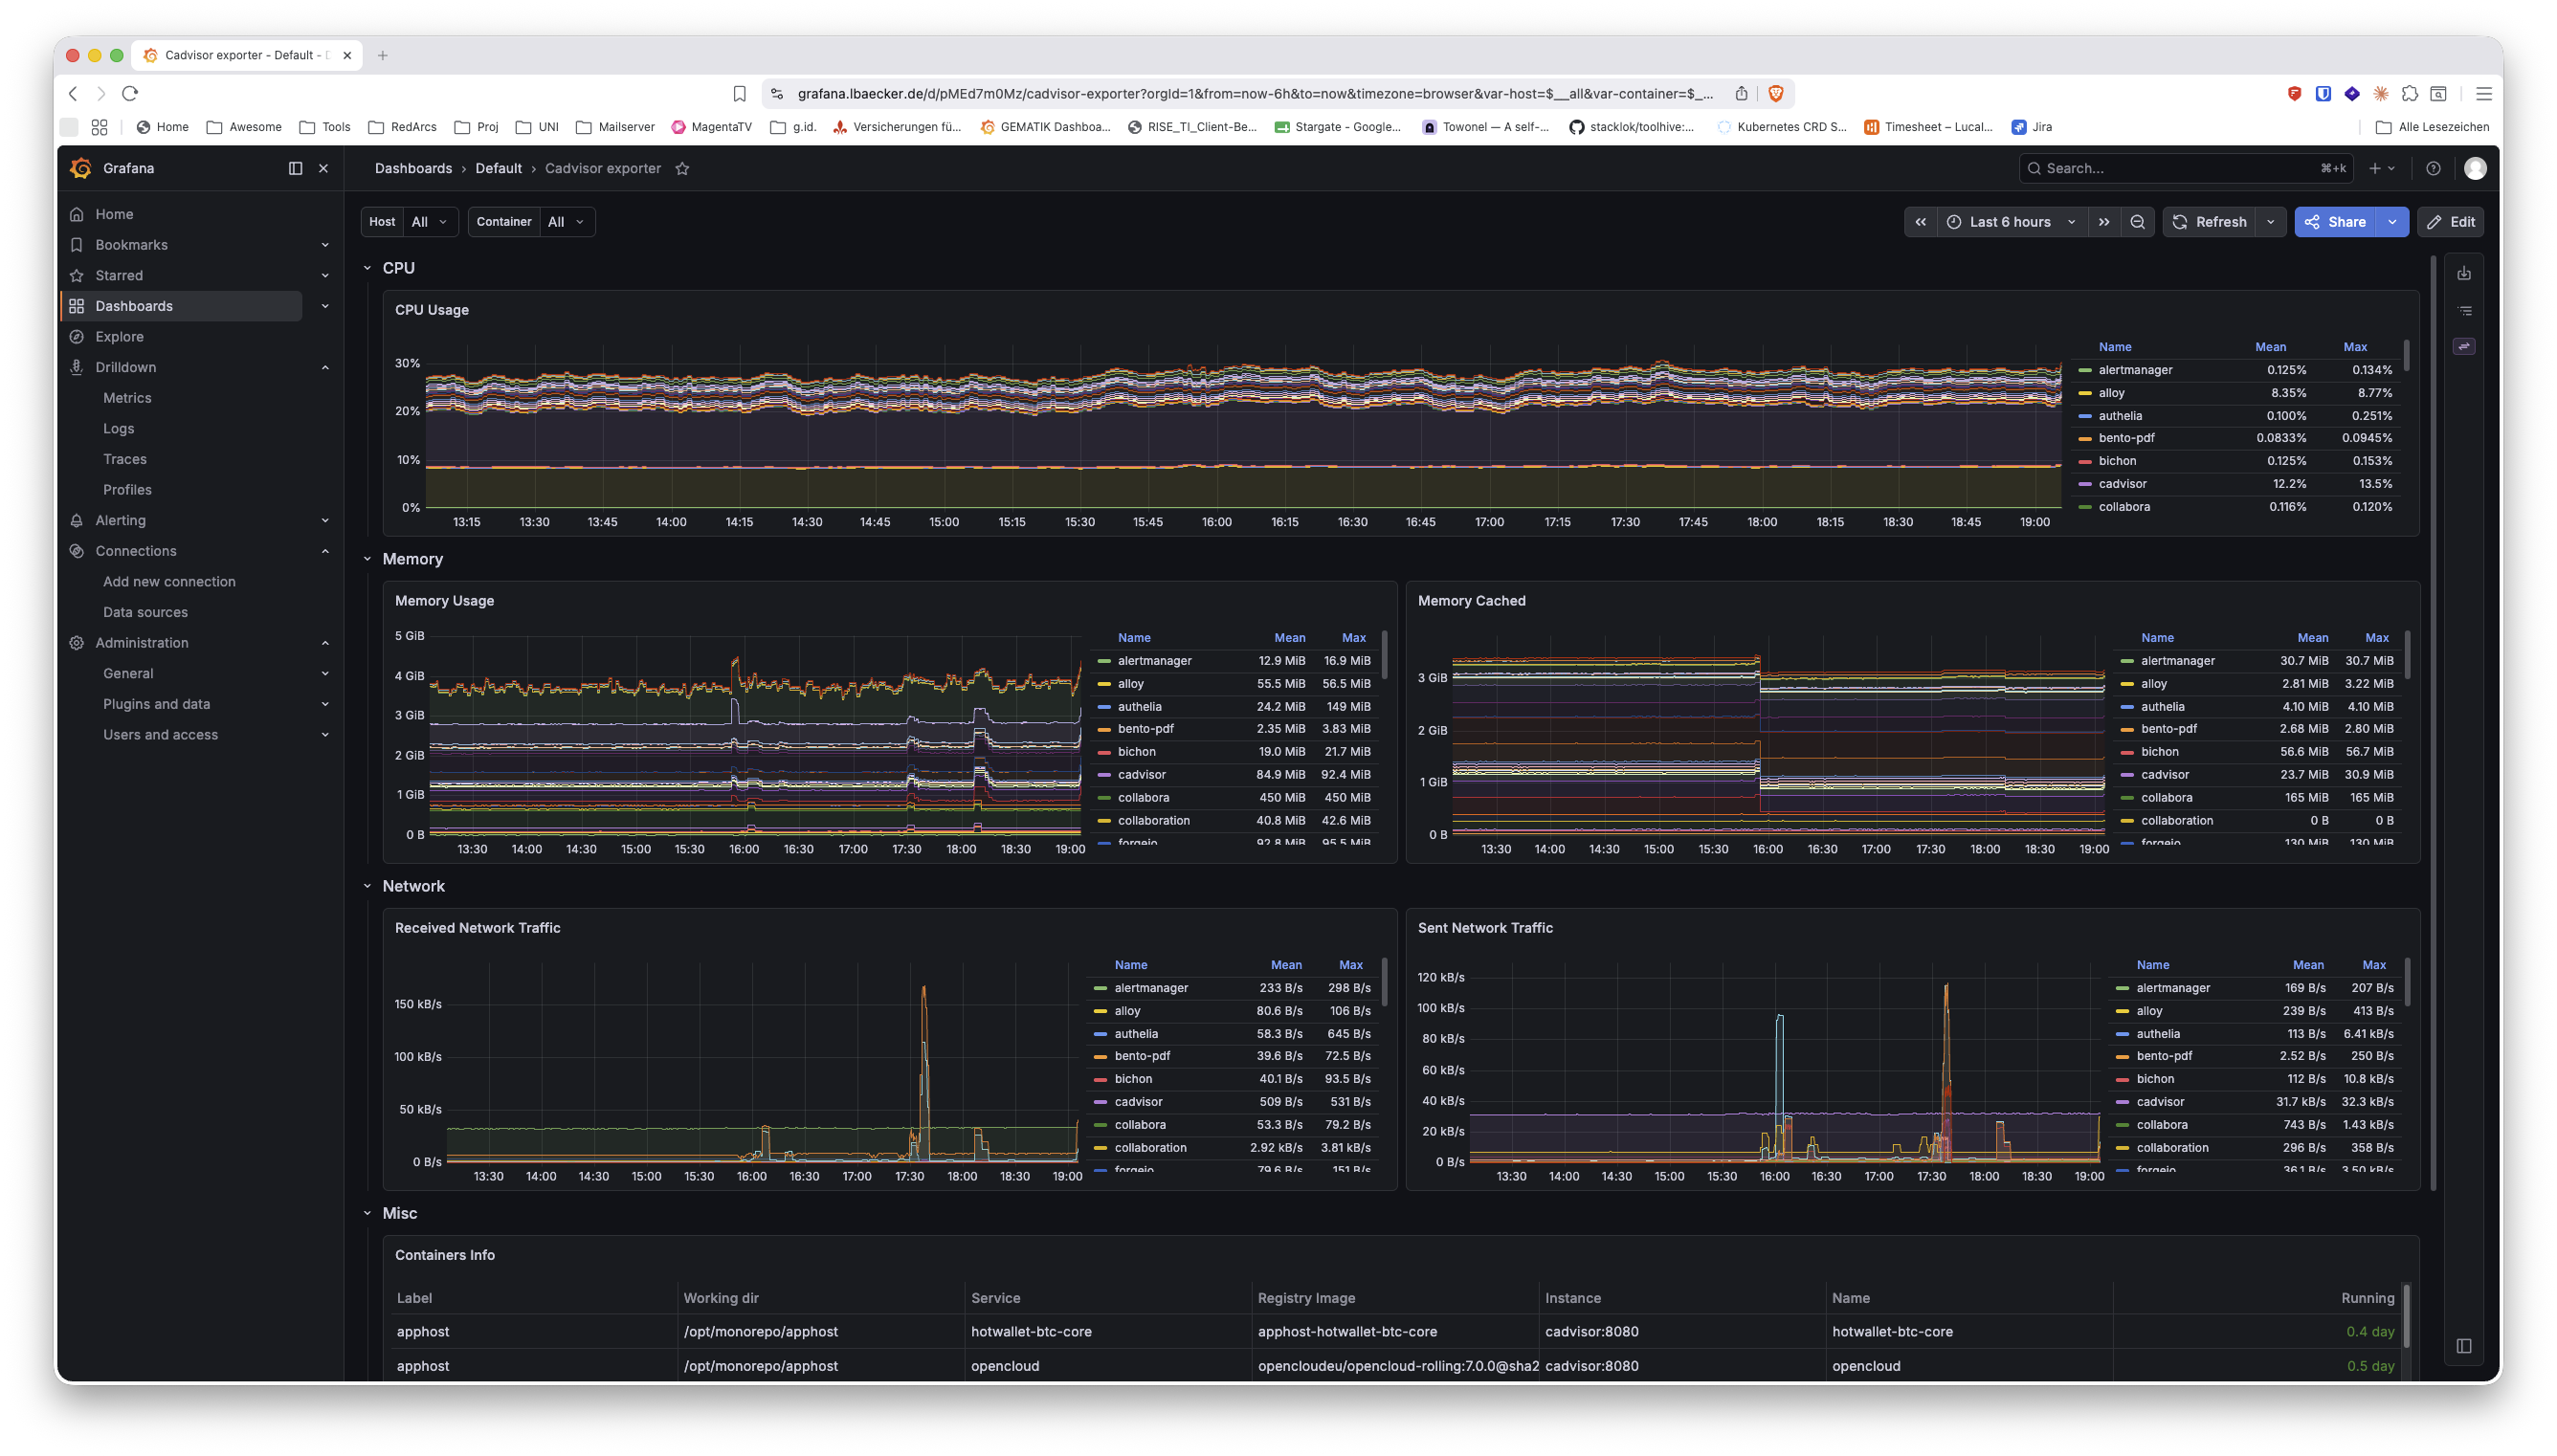
\includegraphics[width=0.9\textwidth]{Doku/Apphost/bilder/grafana_cadvisor_dashboard.png}
    \caption{Grafana-Dashboard \enquote{Cadvisor exporter} mit \acs{CPU}-, Speicher- und Netzwerkauslastung der einzelnen Container sowie einer tabellarischen Übersicht der laufenden Container inklusive Image und Laufzeit. Quelle: Eigene Bildschirmaufnahme.}
    \label{fig:apphost_grafana_cadvisor}
\end{figure}

\begin{figure}[htbp]
    \centering
    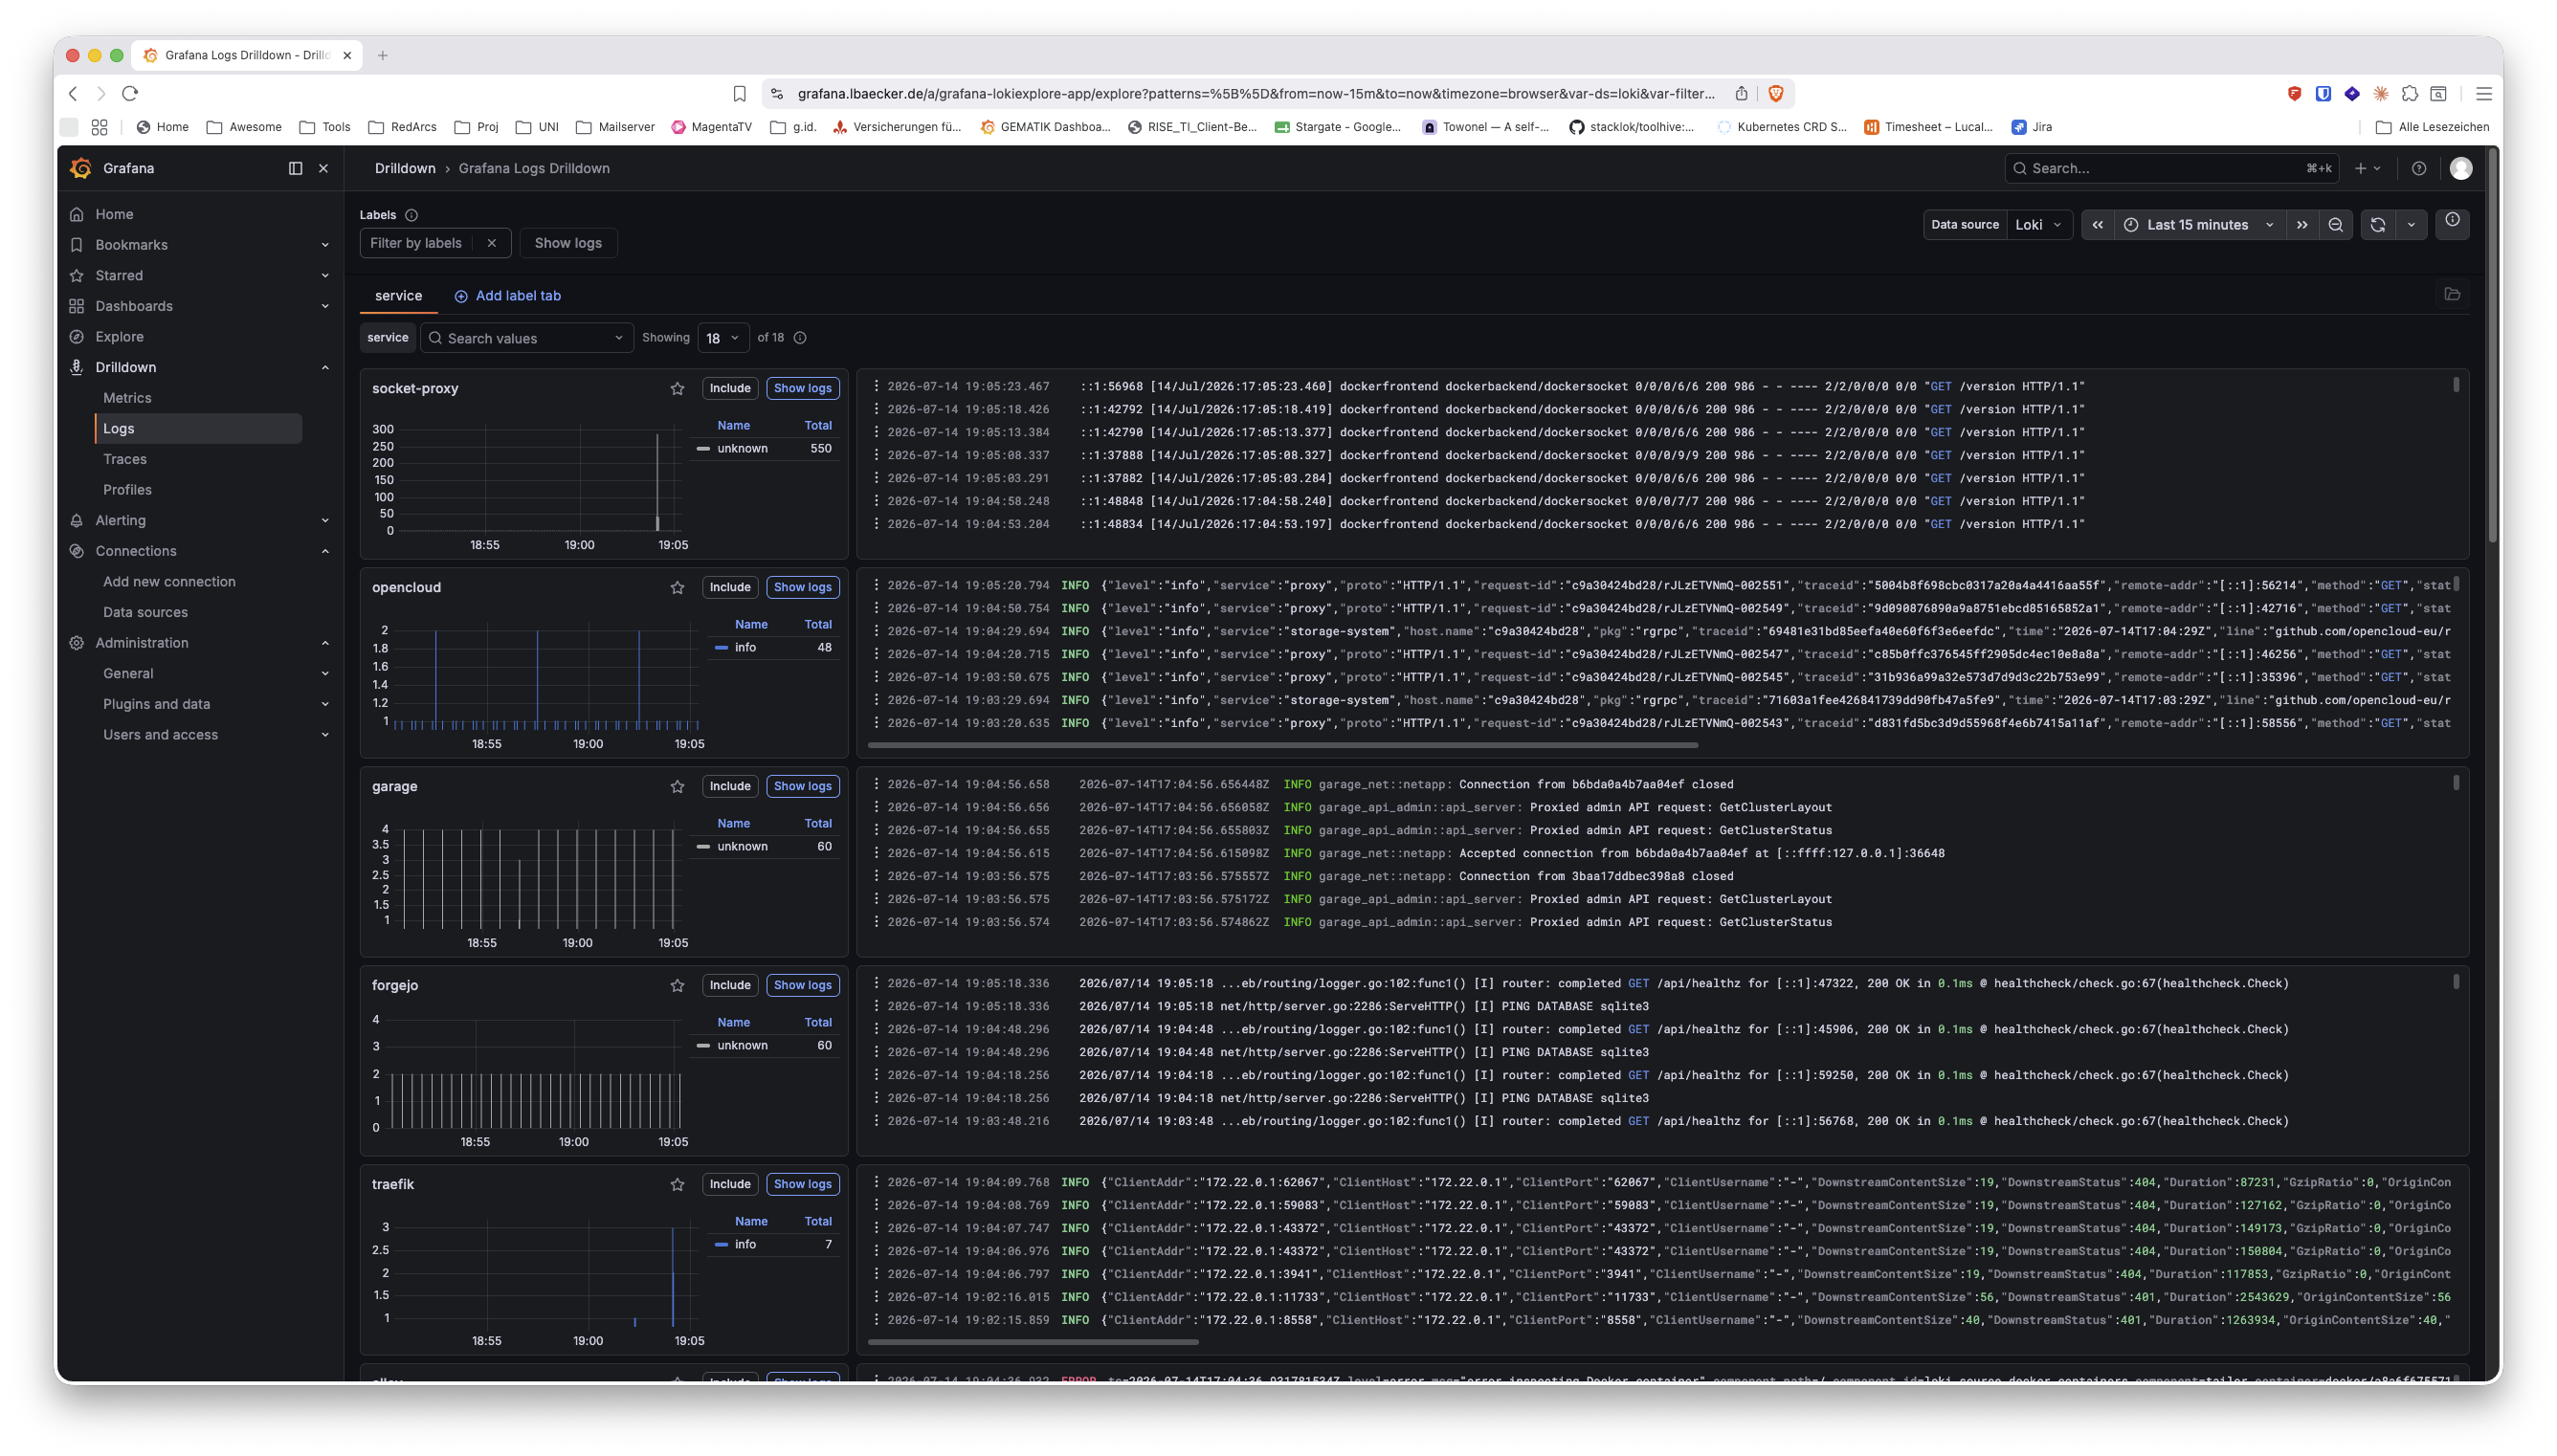
\includegraphics[width=0.9\textwidth]{Doku/Apphost/bilder/grafana_logs_drilldown.png}
    \caption{Grafana-\enquote{Logs Drilldown} auf Basis von Loki, hier gefiltert nach dem Label \texttt{service} mit Log-Volumen und Log-Zeilen je Dienst (u.\,a. \texttt{socket-proxy}, \texttt{opencloud}, \texttt{garage}, \texttt{forgejo}, \texttt{traefik}). Quelle: Eigene Bildschirmaufnahme.}
    \label{fig:apphost_grafana_logs}
\end{figure}

\begin{figure}[htbp]
    \centering
    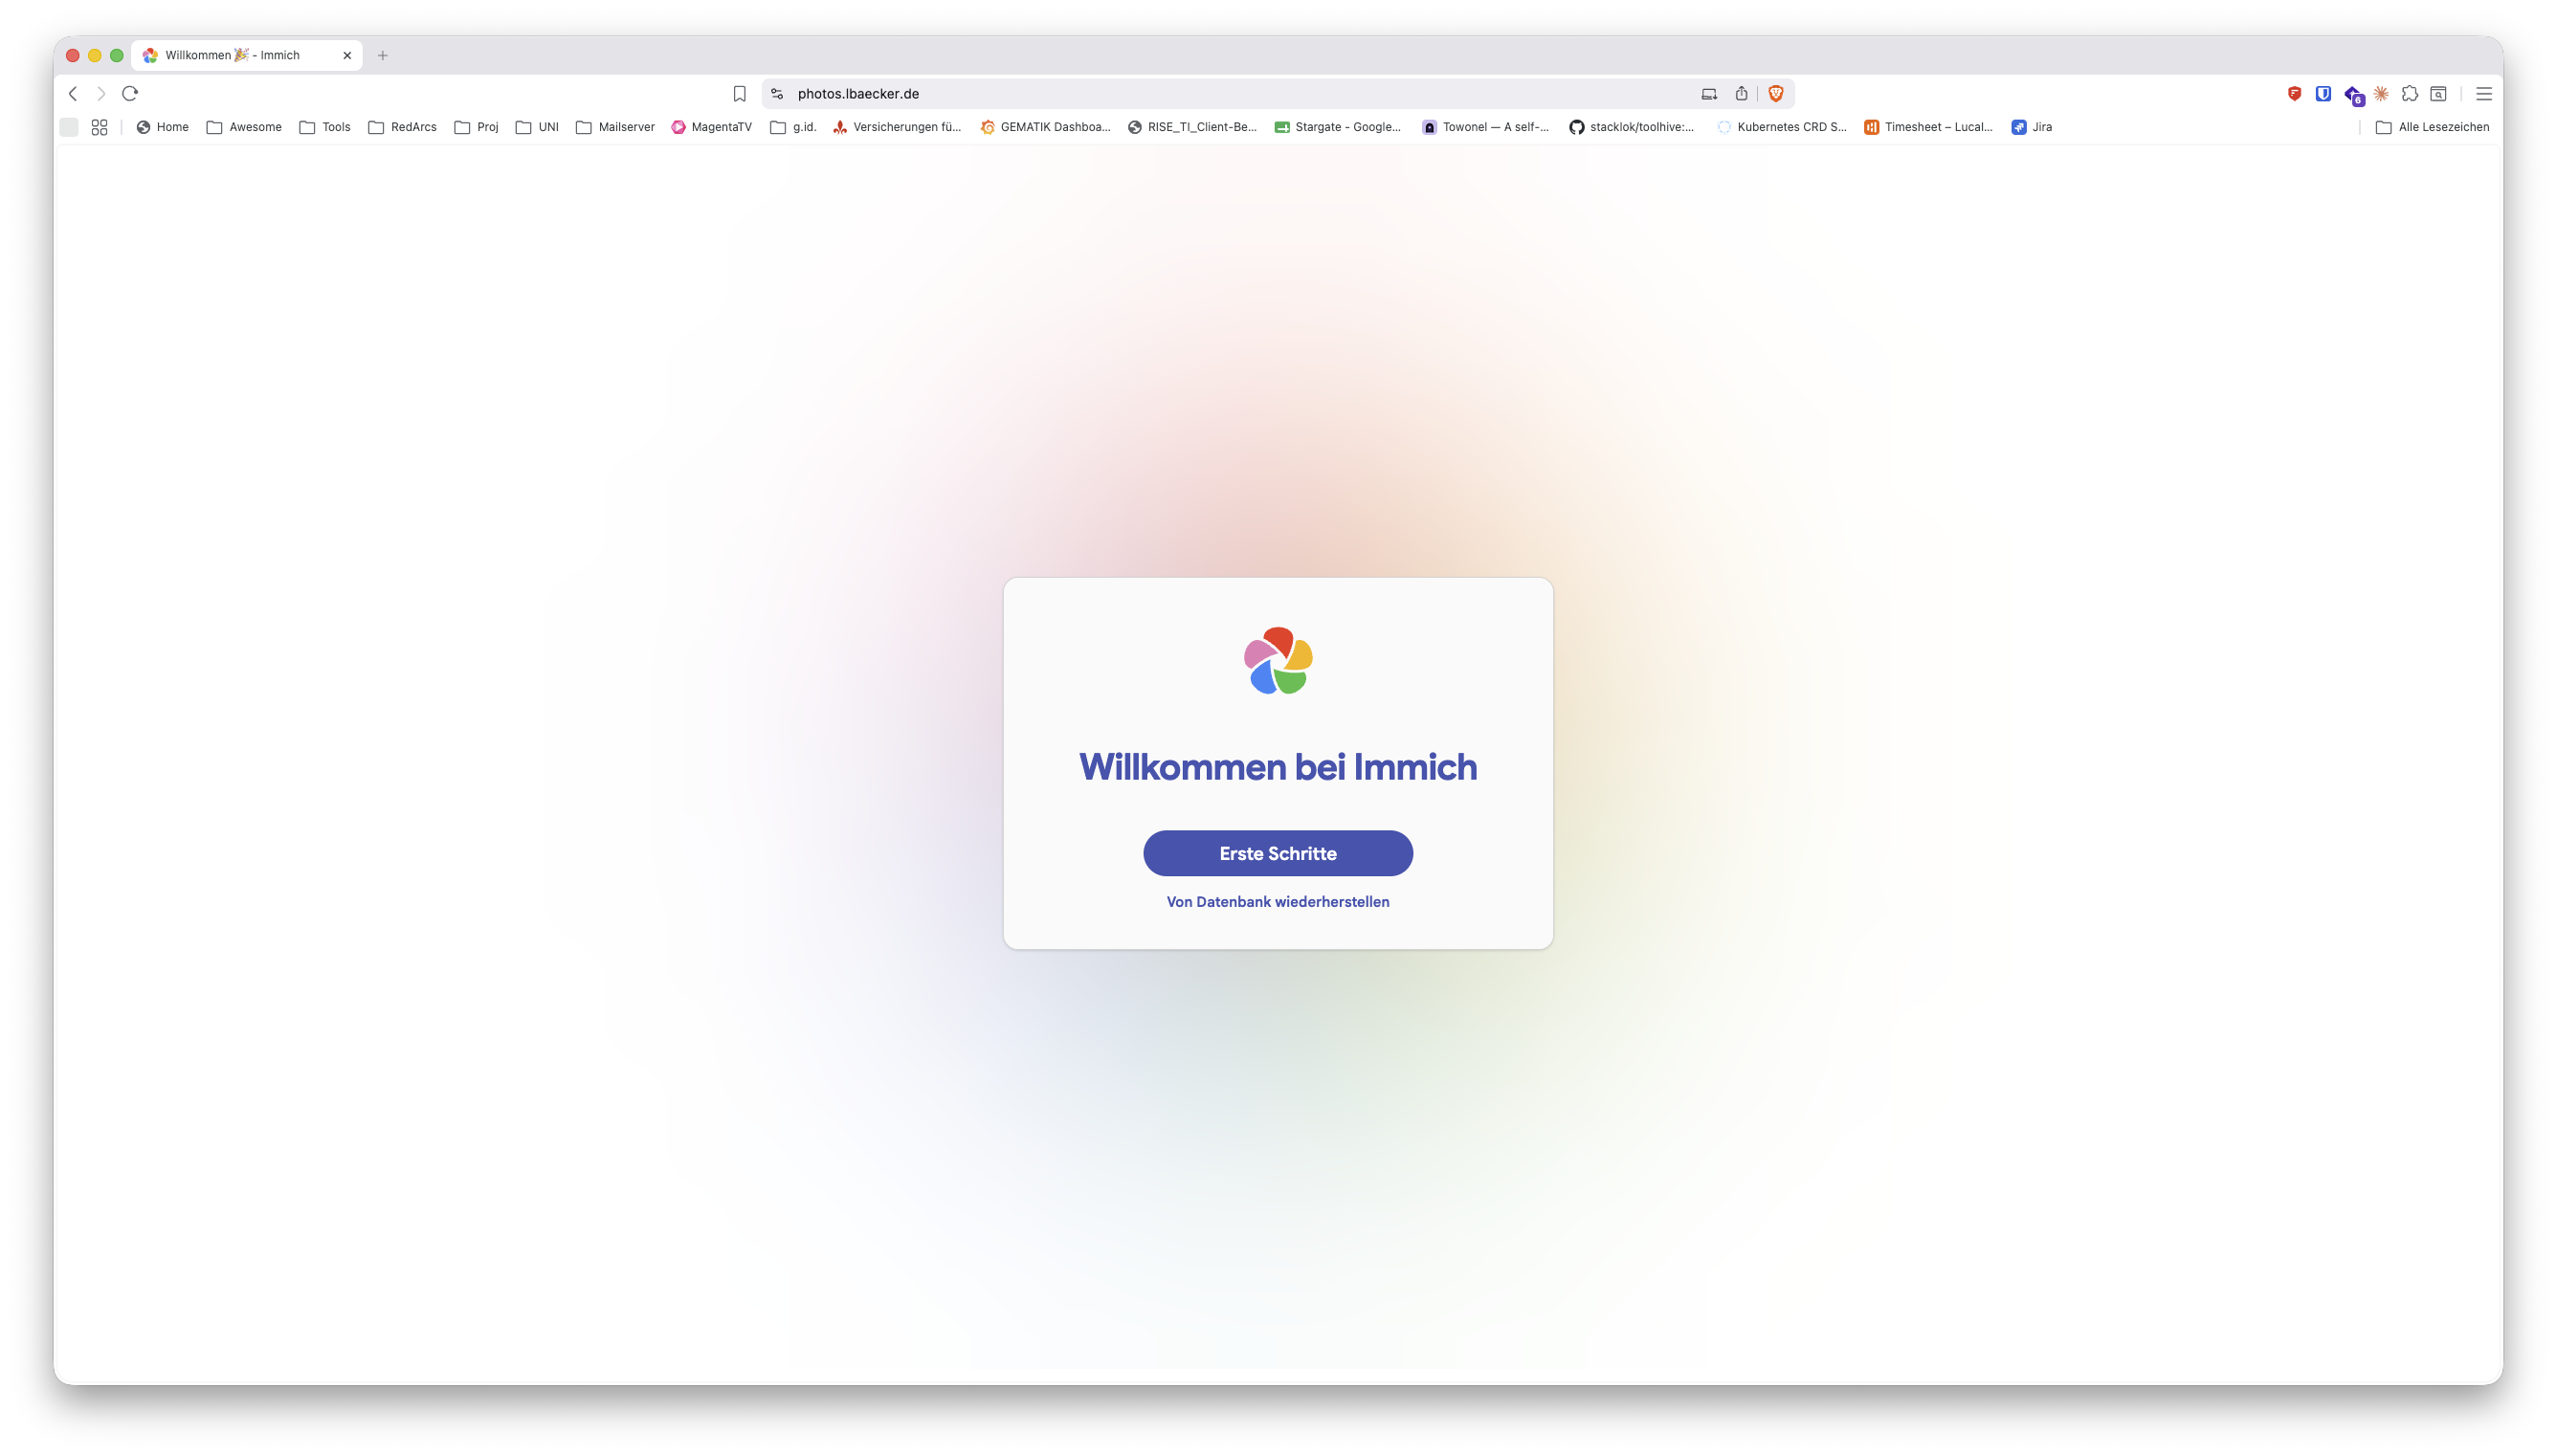
\includegraphics[width=0.7\textwidth]{Doku/Apphost/bilder/immich_welcome.png}
    \caption{Startseite von Immich (\texttt{photos.*}) nach erfolgreicher Bereitstellung. Quelle: Eigene Bildschirmaufnahme.}
    \label{fig:apphost_immich}
\end{figure}

\begin{figure}[htbp]
    \centering
    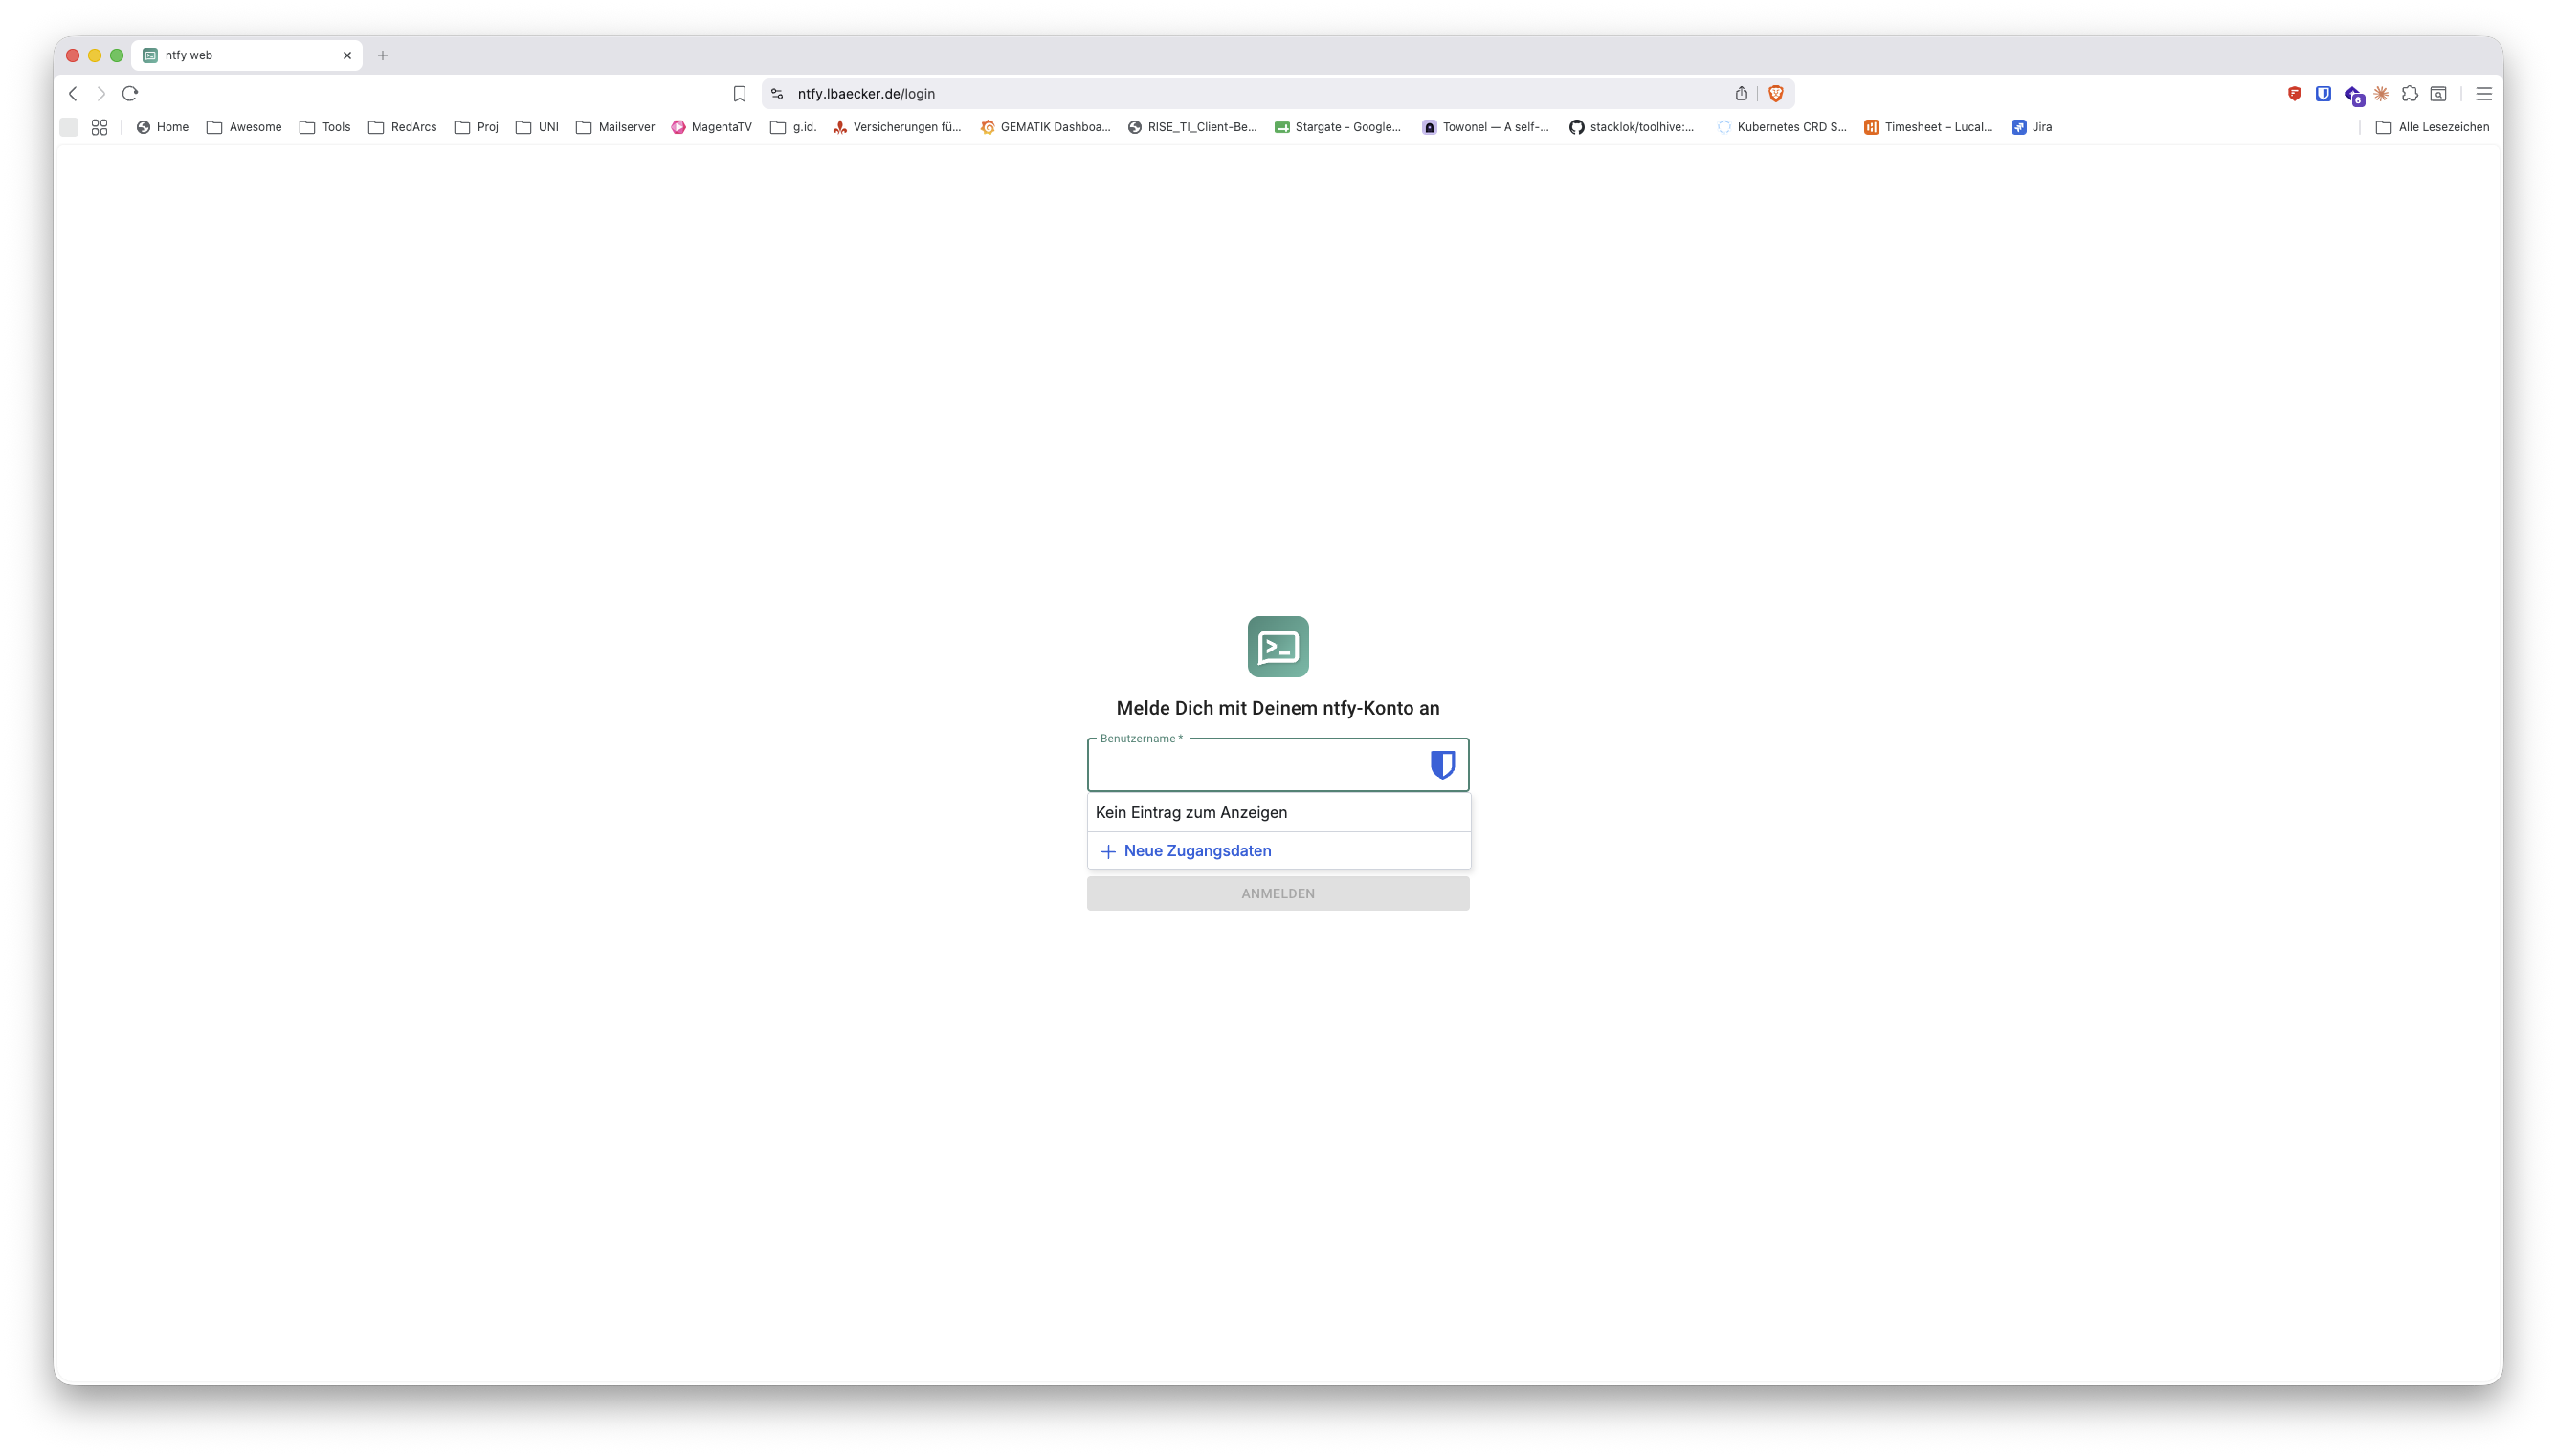
\includegraphics[width=0.7\textwidth]{Doku/Apphost/bilder/ntfy_login.png}
    \caption{Login-Maske der Ntfy-Weboberfläche (\texttt{ntfy.*}) für Push-Benachrichtigungen. Quelle: Eigene Bildschirmaufnahme.}
    \label{fig:apphost_ntfy}
\end{figure}

\begin{figure}[htbp]
    \centering
    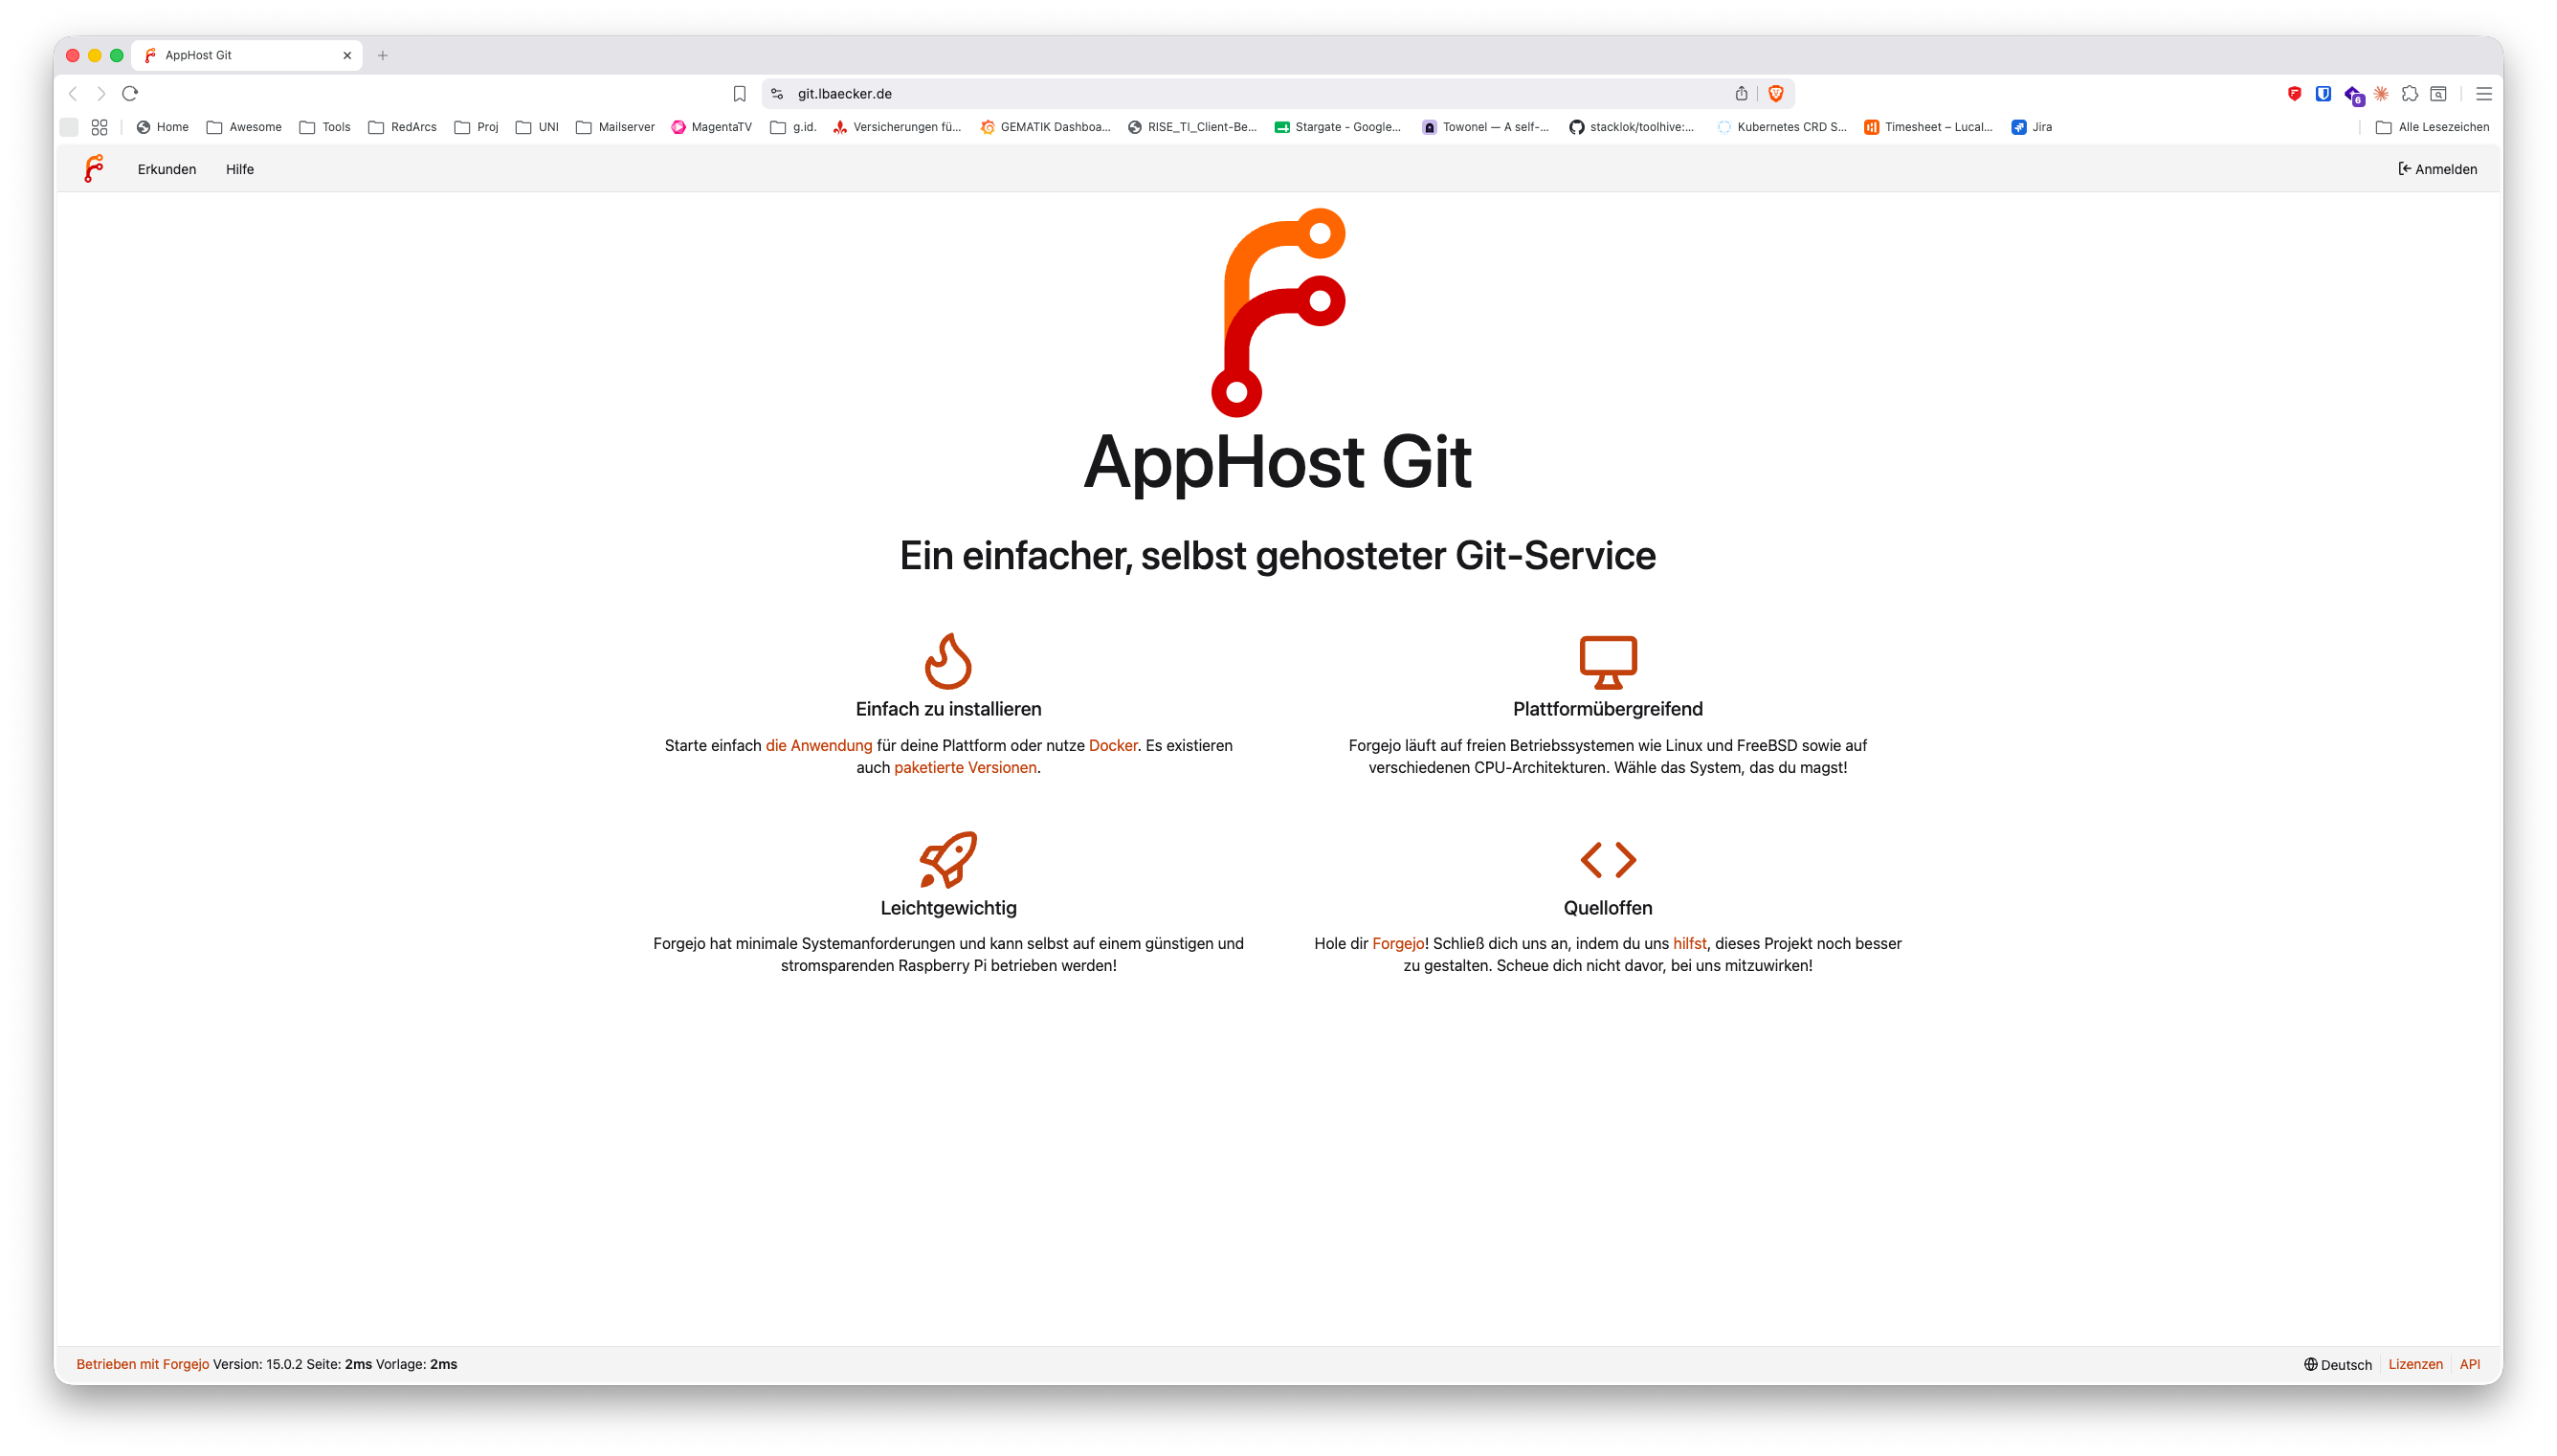
\includegraphics[width=0.7\textwidth]{Doku/Apphost/bilder/forgejo_landing.png}
    \caption{Startseite der selbst gehosteten Git-Plattform Forgejo (\texttt{git.*}, hier unter dem Namen \enquote{AppHost Git}). Quelle: Eigene Bildschirmaufnahme.}
    \label{fig:apphost_forgejo}
\end{figure}

\begin{figure}[htbp]
    \centering
    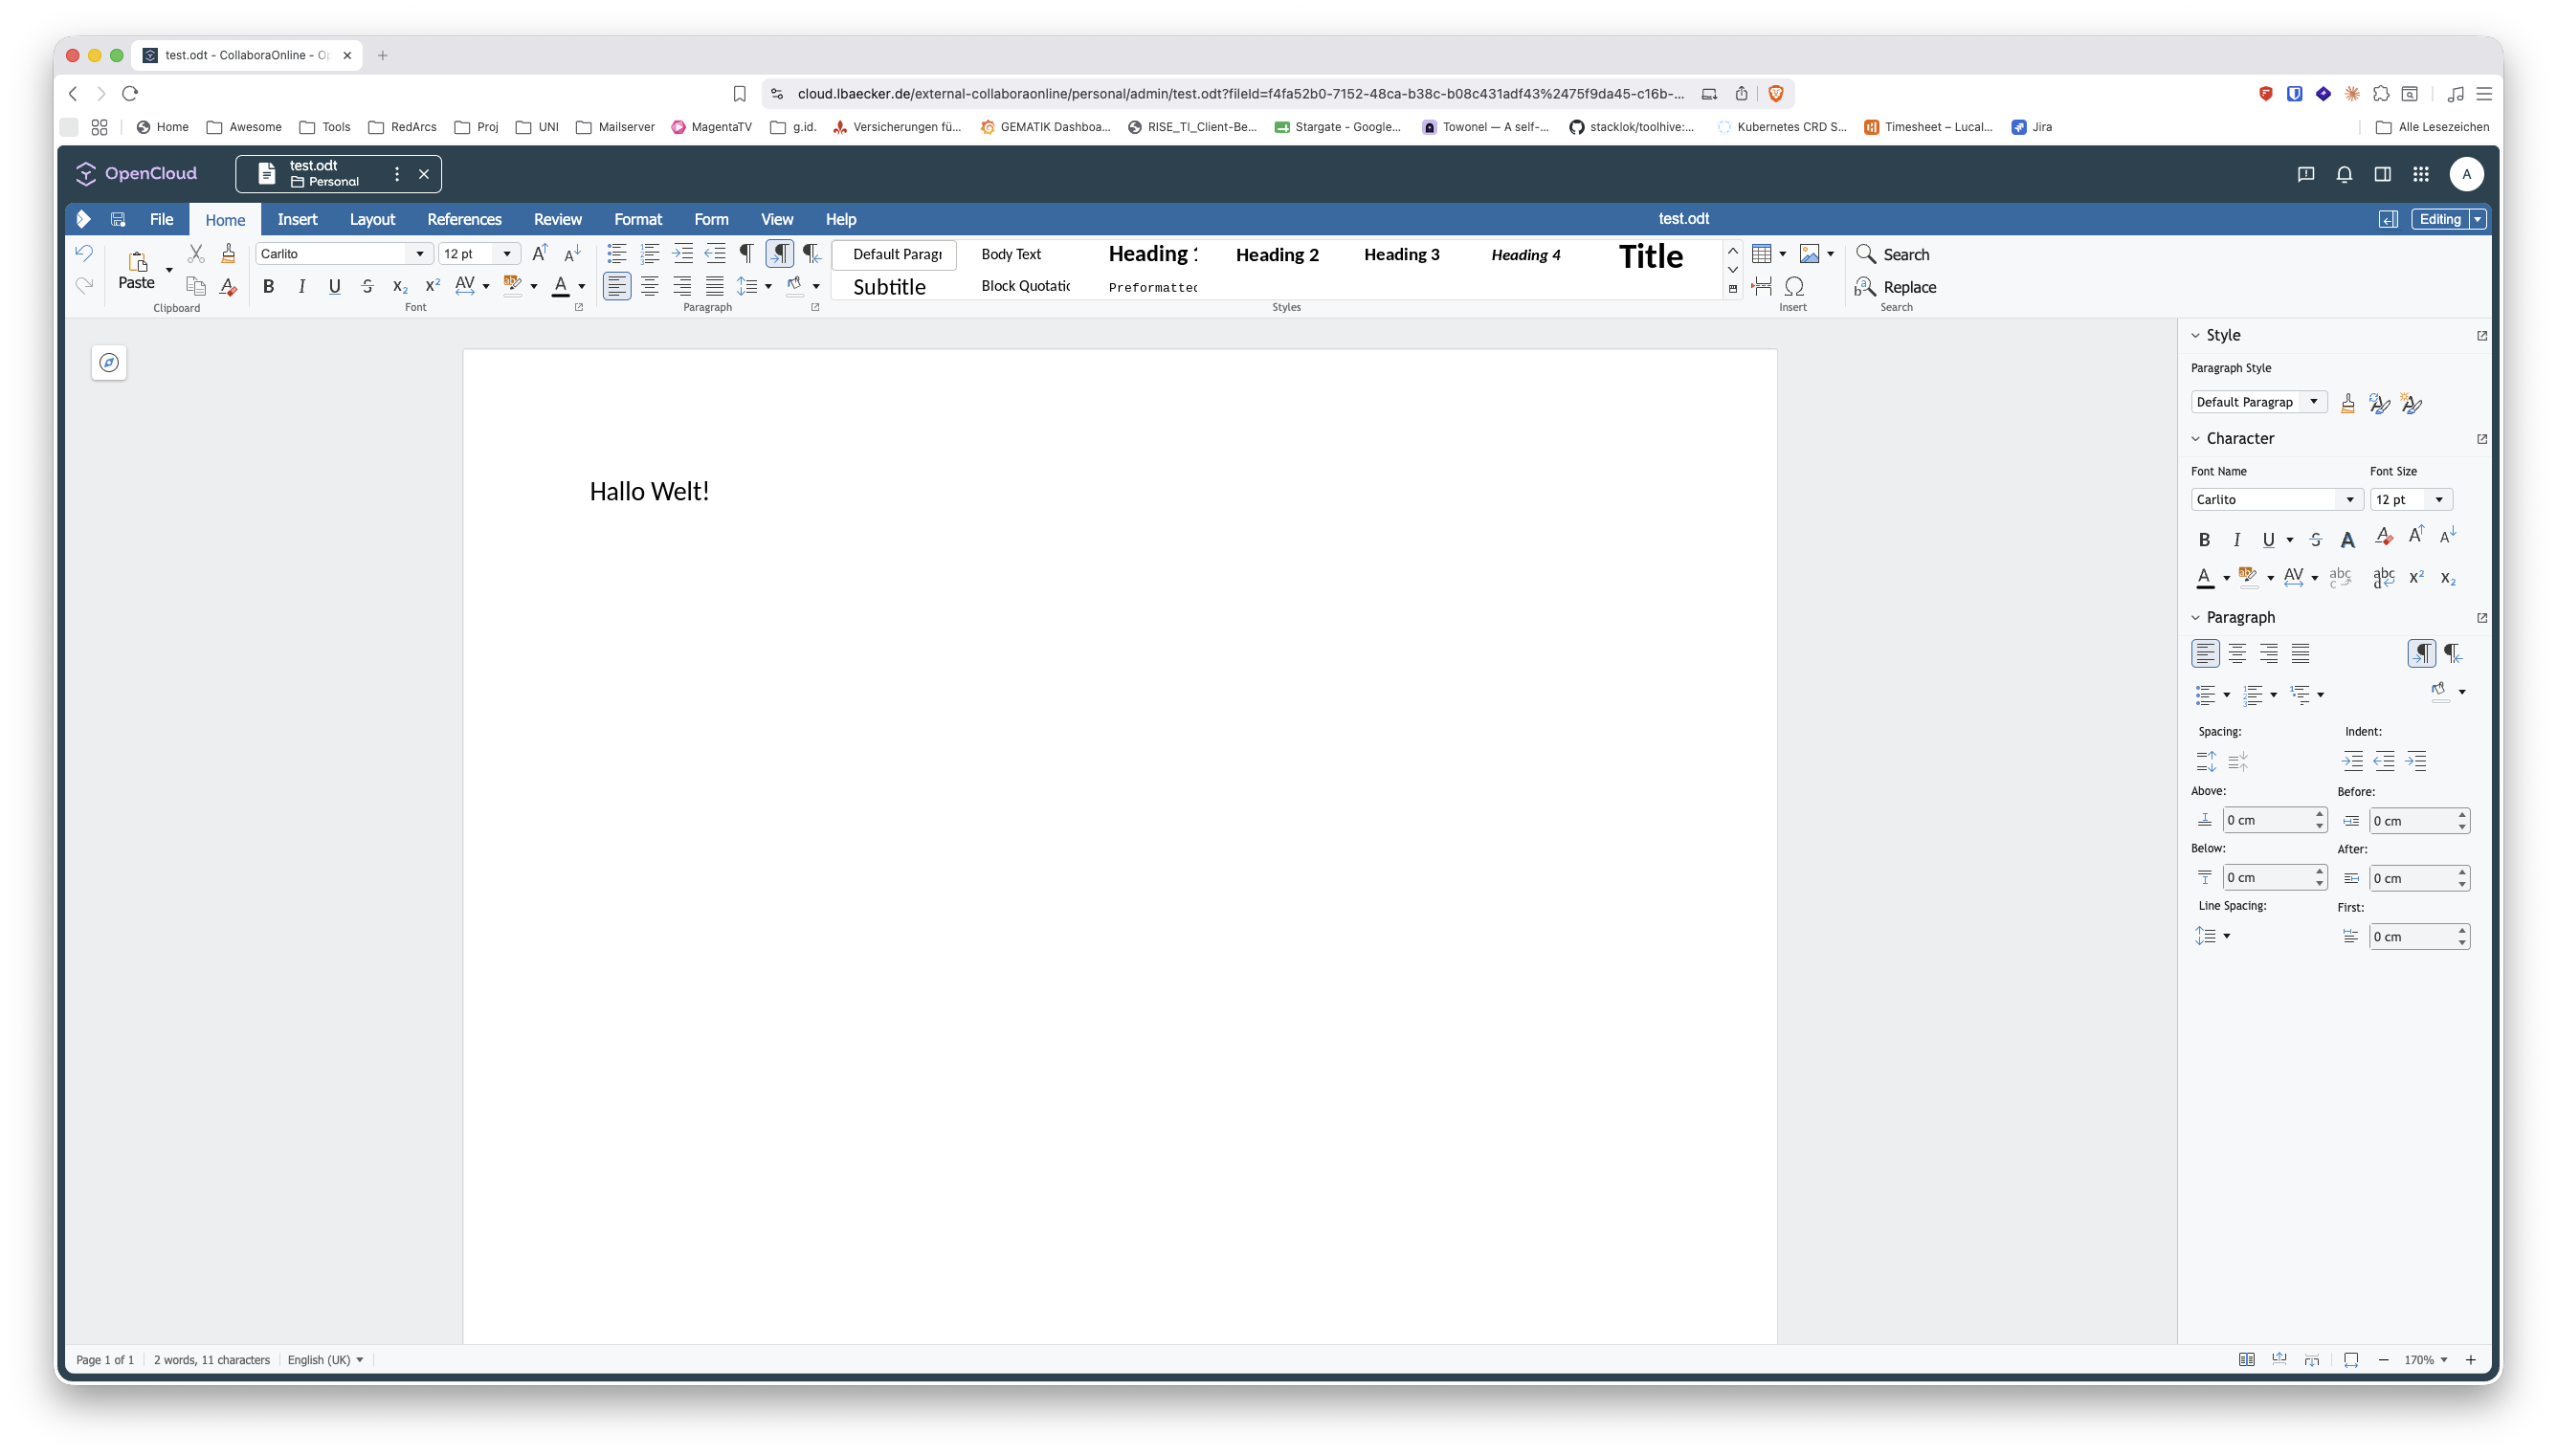
\includegraphics[width=0.9\textwidth]{Doku/Apphost/bilder/opencloud_collabora_editor.png}
    \caption{In OpenCloud (\texttt{cloud.*}) eingebettete Collabora-Online-Bearbeitung einer \texttt{.odt}-Datei über den \acs{WOPI}-Server. Quelle: Eigene Bildschirmaufnahme.}
    \label{fig:apphost_opencloud_collabora}
\end{figure}
